\mychapter{Resultados parciais}
\label{cap:resultados}

\begin{comment}
Neste capítulo será realizada uma análise comparativa dos resultados obtidos nas
duas propostas do sistema de DDF. Ao final, do capítulo a melhor estrutura será
escolhida para que seja feita uma análise mais detalhada dos resultados.
\end{comment}

Neste capítulo serão analisados os resultados parciais obtidos a partir da
implementação da segunda proposta do sistema de DDF. Para isso, em um primeiro
momento será mostrado como se deu a coleta dos dados de treinamento e validação
das redes especialistas e em seguida será feita uma comparação de desempenho. Ao
final do capítulo as melhores estruturas serão selecionadas para que se realize
uma análise um pouco mais detalhada acerca da detecção das falhas.

% ------------------------------------------------------------------------------
\section{Coleta dos dados}
Tanto para o processo de identificação quanto para o processo de detecção, o
primeiro passo a ser dado é a obtenção das amostras experimentais para o
treinamento supervisionado das redes neurais de inferência e de detecção.

Dessa maneira, realizou-se a coleta dos dados a partir da estimulação do sistema
simulado através da aplicação de sinais binários pseudo aleatórios ({Pseudo
Random Binary Signals} -- PRBS) à referência de cada um dos tanques e aos
parâmetros do sistema que simulam as falhas. Para a identificação, a faixa de
valores aplicados se deu do nível mínimo (zero) ao máximo (trinta). Já para a
detecção das falhas, os valores foram aplicados conforme Tab.
\ref{tab:valores_treinamento}. Nessa tabela os valores mínimos e máximos são
multiplicados pelo valor padrão e aplicados ao modelo. A última coluna mostra
qual será a representatividade da mudança dos valores.

\begin{table}[htb]
\small
\caption{Valores aplicados para o treinamento das redes neurais de detecção.}
\label{tab:valores_treinamento}
\vspace{0.25cm}
\centering
\begin{threeparttable}
\begin{tabular}{|c|c|c|c|c|}
\hline
{\bf Falha} & {\bf Valor padrão} & {\bf Mínimo} & {\bf Máximo} & 
{\bf Representatividade}\\
\hline
\hline
FSeDG & 0,16\tnote{$*$} & 
0,8 & 1,2 & Até $\pm 6$ cm\\
\hline
FSeDO & 1,0 & -3,0 & 3,0 & Até $\pm 3$ cm\\
\hline
FSeSR & 1,0 & -0,03 & 0,03 & Até $\pm 9$ cm\\
\hline
FSeQ & 1,0 & 0,0 & 0,0 & -- \\
\hline
\hline
FADG & 1,0 & 0,8 & 1,0 & Até -3 Volts\\
\hline
FADO & 1,0 & -1,0 & 0,0 & Até -1 Volts\\
\hline
FASR & 1,0 & -0,03 & 0,03 & Até $\pm 0,45$ Volts\\
\hline
FAVK & $K_m$ & 0,7 & 1,1 & --\\
\hline
FAQ & 1,0 & 0,0 & 0,0 & --\\
\hline
\hline
FSiVzT & $a_{i_{\text{\tiny MED}}}$ & 
0,25 & 0,75 & 25 a 75\% de $a_{i_{\text{\tiny MED}}}$\\
\hline
FSiVrOS & $a_{i_{\text{\tiny MED}}}$ & 
0,75 & 1,25 & $\pm 25\%$ de $a_{i_{\text{\tiny MED}}}$\\
\hline
FSiVrGMP & 5,0\tnote{$*$} & 
0,8 & 1,0 & Até -3 Volts\\
\hline
FSiEOS & $a_{i_{\text{\tiny MED}}}$ & 
0,0 & 0,5 & --\\
\hline
\end{tabular}
\begin{tablenotes}
\item [$*$] Estabelecido pelo manual do fabricante.
\end{tablenotes}
\end{threeparttable}
\end{table}

Perceba que nas falhas dos atuadores, as tensões a serem aplicadas podem vir a
danificar a bomba. Por esse motivo não seria viável obter as amostras do
processo real, mas sim a partir de uma simulação.

Os sinais pseudo aleatórios gerados se mantiveram dentro dos limites
estabelecidos durante todo o intervalo de tempo da simulação. Para o processo de
identificação foram obtidas 6000 (seis mil) amostras, equivalentes à 10 (dez)
minutos de simulação. Já para a detecção o processo foi simulado durante 20
(vinte) minutos, o que correspondeu a obtenção de 12000 (doze mil) amostras.

De posse dos valores obtidos, iniciou-se a fase de treinamento das RNAs. Todas
as redes foram treinadas de modo {\it offline} com o {\it toolbox} de redes
neurais do {\it software} matemático Matlab\reg\ utilizando o algoritmo LMA. Ao
final de cada etapa de treinamento as redes eram submetidas à testes de
validação para que se fosse possível avaliar a capacidade de generalização.

% ------------------------------------------------------------------------------
\section{Análise das RNAs}
Para que se fossem estabelecidos critérios avaliativos significantes, ou seja,
para que existisse um número representativo, diversas redes neurais foram
treinadas com diferentes configurações do número de neurônios na camada oculta e
da ordem do modelo. O número de redes treinadas corresponde aquele especificado
no final da Tab. \ref{tab:treinamentos}. 

\begin{table}[htb]
\small
\centering
\caption[Número de redes neurais treinadas]{Número de redes neurais treinadas de
acordo com a ordem do modelo e o número de neurônios na camada oculta.}
\label{tab:treinamentos}
\vspace{0.25cm}
\begin{tabular}{|c|c|c|c|c|}
\hline
% Linha 1
\multirow{2}{*}{\bf Proposta} & 
\multirow{2}{*}{\bf Ordem} & 
{\bf Neurônios na} & 
{\bf Número de} & 
\multirow{2}{*}{\bf Total}\\
% Linha 2
& & {\bf camada oculta} & {\bf redes treinadas} &\\
\hline
\hline
\multicolumn{5}{|l|}{{\bf Identificação}}\\
\hline
\multirow{3}{*}{1} & 2 & 6/8/10 & \multirow{3}{*}{6} & \multirow{3}{*}{54}\\
\cline{2-3}
& 3 & 8/12/16 & &\\
\cline{2-3}
& 4 & 10/16/22 & &\\
\hline
\multirow{3}{*}{2} & 2 & 2/4/6 -- 6/8/10 & 
\multirow{3}{*}{6} & \multirow{3}{*}{108}\\
\cline{2-3}
& 3 & 4/6/8 -- 8/12/16 & & \\
\cline{2-3}
& 4 & 6/8/10 -- 10/16/22 & & \\
\hline
\multicolumn{5}{|l|}{{\bf Detecção}}\\
\hline
\multirow{3}{*}{2} & 2 & 8/12/16 & 
\multirow{3}{*}{6/falha} &
\multirow{3}{*}{702}\\
\cline{2-3}
& 3 & 14/18/22 & &\\
\cline{2-3}
& 4 & 20/24/28 & &\\
\hline
\hline
\multicolumn{4}{|r|}{{\bf Total}} & 864\\
\hline
\end{tabular}
\end{table}

Na primeira proposta de identificação, de segunda ordem, foram treinadas 6
(seis) redes neurais cada vez que o número de neurônios na camada oculta era
alterado. Ou seja, para cada ordem eram treinadas 18 (dezoito) redes neurais.
Como foram testadas três ordens distintas em cada proposta, tem-se um total de
54 (cinquenta e quatro) redes para a primeira proposta.

Observa-se entretanto que, na segunda proposta de identificação existiam duas
redes neurais a serem treinadas em cada etapa de treinamento, conforme Fig.
\ref{fig:ident_proposta_2}, e que a segunda proposta de detecção considera-se um
conjunto de 13 (treze) redes especialistas, sendo uma para cada falha, conforme
Fig. \ref{fig:detec_prop_2}. Em virtude desses aspectos, o número de redes
treinadas dobra da primeira para a segunda proposta de identificação e é
multiplicado por um fator de treze para a segunda proposta de detecção.

% ------------------------------------------------------------------------------
\section{Melhores redes}
Diante do grande número de redes neurais a serem analisadas, foi necessário
estabelecer algum tipo de critério avaliativo para que as melhores redes fossem
selecionadas. Para as propostas de detecção utilizou-se o EMQ sobre os valores
de saída $\widehat{L_1}$ e $\widehat{L_2}$, enquanto que para as redes de
detecção fez-se uso do número de erros de tipo I e erros de tipo II.  O EMQ e o
número de erros de tipo I e II de cada rede foram obtidos a partir da média dos
valores de três validações distintas.

% ------------------------------------------------------------------------------
\subsection{Redes para identificação}
Utilizando o EMQ estabelecido pela Eq. \ref{eq:emq}, foram obtidos os resultados
exibidos pela Tab. \ref{tab:melhores_rnas_ident}.

\begin{table}[htb]
\small
\centering
\caption{Melhores redes treinadas para a identificação do modelo.}
\label{tab:melhores_rnas_ident}
\vspace{0.25cm}
\begin{threeparttable}
\begin{tabular}{|c|c|c|c|c|c|c|}
\hline
% Linha 1
{\bf Proposta} & 
{\bf Ordem} & 
{\bf NCO\tnote{$*$}} & 
{\bf Treinamento} &
{\bf EMQ $\mathbf{L_1}$} & 
{\bf EMQ $\mathbf{L_2}$} & 
{\bf EMQ}\\
\hline
\hline
\multirow{3}{*}{1} &
\cellcolor[gray]{0.9} 2 &
\cellcolor[gray]{0.9} 8 &
\cellcolor[gray]{0.9}2 &
\cellcolor[gray]{0.9} 4,39e-7 &
\cellcolor[gray]{0.9} 3,29e-6 &
\cellcolor[gray]{0.9} 3,73e-6\\
\cline{2-7}
&3 & 12 & 5 & 1,38e-5 & 1,46e-5 & 2,84e-5\\
\cline{2-7}
&4 & 22 & 4 & 1,40e-6 & 2,60e-6 & 4,01e-6\\
\hline
\multirow{3}{*}{2} & 2 & 2 -- 6 & 2 & 5,06e-6 & 7,26e-6 & 1,23e-5\\
\cline{2-7}
& 3 & 6 -- 12 & 1 & 5,48e-6 & 1,81e-7 & 5,66e-6\\
\cline{2-7}
& 4 & 10 -- 22 & 3 & 5,12e-6 & 9,46e-6 & 1,45e-5\\
\hline
\end{tabular}
\begin{tablenotes}
\item [$*$] Número de neurônios na camada oculta.
\end{tablenotes}
\end{threeparttable}
\end{table}

Assim, a melhor rede de identificação, escolhida para estimar os valores de
$L_1$ e $L_2$, foi a rede de segunda ordem, com oito neurônios na camada oculta,
obtida no segundo treinamento. Essa rede, cuja soma dos EMQs foi de $3,73 \times
10^{-6}$, será utilizada para gerar os valores dos resíduos ($e_i = L_i -
\widehat{L_i}$) que compõem a entrada das redes de detecção.

% ------------------------------------------------------------------------------
\subsection{Redes para detecção de falhas}
De maneira simplificada, pode-se dizer que os erros de tipo I, também conhecidos
como {\it falsos positivos}, ocorrem quando o sistema reconhece uma falha que,
na verdade, não houve, enquanto que os erros de tipo II, também conhecidos como
{\it falsos negativos}, ocorrem quando o sistema deixa de reconhecer uma falha
que aconteceu.

Dessa maneira, a escolha das melhores redes de detecção se deu a partir do
número de incidência de cada um desses erros. Estabeleceu-se portanto que a
melhor rede para uma determinada falha seria aquela em que a soma dos erros de
tipo I com os erros de tipo II fosse a menor possível.

Os resultados obtidos para cada uma das falhas podem ser observados na Tab.
\ref{tab:melhores_redes_detec}. Como dito anteriormente, as colunas dos erros se
referem a média obtida a partir das três validações. Já a última coluna
representa o percentual de erro médio total\footnote{O percentual de erro médio
total é obtido a partir da soma da quantidade de erros de tipo I com os erros de
tipo II, dividido pelo número total de amostras.} sobre todas as amostras. 

Deve-se observar ainda que apesar do treinamento ter sido feito com 12000 (doze
mil) amostras, a rede deve acertar 24000 (vinte e quatro mil) vezes, pois para
cada ponto a rede deve mostrar se está ou não havendo aquela falha em $T_1$ e em
$T_2$. Portanto, para cada ponto de treinamento haverão dois acertos a serem
realizados. Ademais, assim como na proposta de identificação, as melhores redes
estão destacadas em cinza.

\begin{center}
\small
\tablefirsthead
{
\hline
\multirow{2}{*}{\bf Falha} &
\multirow{2}{*}{\bf Ordem} &
\multirow{2}{*}{\bf NCO} &
\multirow{2}{*}{\bf Treinamento} &
\multirow{2}{*}{\bf Acertos} &
{\bf Erros de} & {\bf Erros de} & {\bf Total de}\\
& & & & & {\bf tipo I} & {\bf tipo II} & {\bf erros}\\
\hline
\hline
}
% Demais cabeçalhos
\tablehead
{
\hline
\multicolumn{8}{|l|}{\scriptsize\it Continuação da página anterior}\\
\hline
\multirow{2}{*}{\bf Falha} &
\multirow{2}{*}{\bf Ordem} &
\multirow{2}{*}{\bf NCO} &
\multirow{2}{*}{\bf Treinamento} &
\multirow{2}{*}{\bf Acertos} &
{\bf Erros de} & {\bf Erros de} & {\bf Total de}\\
& & & & & {\bf tipo I} & {\bf tipo II} & {\bf erros}\\
\hline
\hline
}
% Final da tabela em cada página
\tabletail
{
\hline
\multicolumn{8}{|r|}{\scriptsize\it Continua na página seguinte}\\
\hline
}
% Último final da tabela
\tablelasttail
{
\hline
}
\tablecaption{Melhores redes treinadas para a detecção de falhas.}
\label{tab:melhores_redes_detec}
\begin{supertabular}{|c|c|c|c|c|c|c|c|}
\multirow{3}{*}{FSeDG} &
2 & 16 & 1 & 23430 & 133,66 & 436,33 & 2,37\%\\
\cline{2-8}
& 3 & 22 & 6 & 23456,33 & 176 & 367,66 & 2,26\%\\
\cline{2-8}
& 
\cellcolor[gray]{0.9}4 & 
\cellcolor[gray]{0.9}28 & 
\cellcolor[gray]{0.9}2 &
\cellcolor[gray]{0.9}23491,33 & 
\cellcolor[gray]{0.9}203,33 & 
\cellcolor[gray]{0.9}305,33 & 
\cellcolor[gray]{0.9}2,12\%\\
\hline
\multirow{3}{*}{FSeDO} &
2 & 16 & 3 & 23872 & 4,33 & 123,66 & 0,53\%\\
\cline{2-8}
& 3 & 14 & 6 & 23876,33 & 23,66 & 100 & 0,51\%\\
\cline{2-8}
& 
\cellcolor[gray]{0.9}4 & 
\cellcolor[gray]{0.9}28 & 
\cellcolor[gray]{0.9}5 & 
\cellcolor[gray]{0.9}23890,33 & 
\cellcolor[gray]{0.9}8,66 & 
\cellcolor[gray]{0.9}101 & 
\cellcolor[gray]{0.9}0,46\%\\
\hline
\multirow{3}{*}{FSeSR} &
2 & 8 & 2 & 23306,33 & 201 & 492,66 & 2,89\%\\
\cline{2-8}
& 3 & 14 & 5 & 23313,66 & 419 & 267,33 & 2,86\%\\
\cline{2-8}
& 
\cellcolor[gray]{0.9}4 & 
\cellcolor[gray]{0.9}20 & 
\cellcolor[gray]{0.9}3 & 
\cellcolor[gray]{0.9}23317 & 
\cellcolor[gray]{0.9}324,66 & 
\cellcolor[gray]{0.9}358,33 & 
\cellcolor[gray]{0.9}2,84\%\\
\hline
\multirow{3}{*}{FSeQ} &
2 & 12 & 5 & 23972 & 21 & 7 & 0,12\%\\
\cline{2-8}
& 3 & 18 & 4 & 23993 & 1,33 & 5,66 & 0,03\%\\
\cline{2-8}
& 
\cellcolor[gray]{0.9}4 & 
\cellcolor[gray]{0.9}20 & 
\cellcolor[gray]{0.9}4 & 
\cellcolor[gray]{0.9}23994 & 
\cellcolor[gray]{0.9}0,66 & 
\cellcolor[gray]{0.9}5,33 & 
\cellcolor[gray]{0.9}0,02\%\\
\hline
\multirow{3}{*}{FADG} &
\cellcolor[gray]{0.9}2 & 
\cellcolor[gray]{0.9}8 & 
\cellcolor[gray]{0.9}3 & 
\cellcolor[gray]{0.9}20710,33 & 
\cellcolor[gray]{0.9}1626,66 & 
\cellcolor[gray]{0.9}1663 & 
\cellcolor[gray]{0.9}13,7\%\\
\cline{2-8}
& 3 & 14 & 6 & 20465 & 1734 & 1801 & 14,73\%\\
\cline{2-8}
& 4 & 20 & 2 & 20116 & 2075,66 & 1808,33 & 16,18\%\\
\hline
\multirow{1}{*}{FADO} &
2 & 12 & 2 & 22827,66 & 612 & 560,33 & 4,88\%\\
\multirow{2}{*}{FADO} &
3 & 22 & 6 & 22903,33 & 606,33 & 490,33 & 4,57\%\\
\cline{2-8}
& 
\cellcolor[gray]{0.9}4 & 
\cellcolor[gray]{0.9}28 & 
\cellcolor[gray]{0.9}3 & 
\cellcolor[gray]{0.9}23075,33 & 
\cellcolor[gray]{0.9}635,66 & 
\cellcolor[gray]{0.9}289 & 
\cellcolor[gray]{0.9}3,85\%\\
\hline
\multirow{3}{*}{FASR} &
\cellcolor[gray]{0.9}2 & 
\cellcolor[gray]{0.9}8 & 
\cellcolor[gray]{0.9}6 & 
\cellcolor[gray]{0.9}14153,33 & 
\cellcolor[gray]{0.9}3407 & 
\cellcolor[gray]{0.9}6439,66 & 
\cellcolor[gray]{0.9}41,03\%\\
\cline{2-8}
& 3 & 14 & 6 & 13977,33 & 4064 & 5958,66 & 41,76\%\\
\cline{2-8}
& 4 & 20 & 3 & 13578,33 & 4393,66 & 6028 & 43,42\%\\
\hline
\multirow{3}{*}{FAVK} &
\cellcolor[gray]{0.9}2 & 
\cellcolor[gray]{0.9}8 & 
\cellcolor[gray]{0.9}5 & 
\cellcolor[gray]{0.9}20764,66 & 
\cellcolor[gray]{0.9}1551,33 & 
\cellcolor[gray]{0.9}1684 & 
\cellcolor[gray]{0.9}13,48\%\\
\cline{2-8}
& 3 & 14 & 5 & 20701,66 & 1336 & 1962,33 & 13,74\%\\
\cline{2-8}
& 4 & 20 & 4 & 20489,33 & 1640,66 & 1870 & 14,63\%\\
\hline
\multirow{3}{*}{FAQ} &
2 & 12 & 6 & 23976 & 0,66 & 23,33 & 0,1\%\\
\cline{2-8}
& 3 & 18 & 2 & 23979,33 & 2,66 & 18 & 0,086\%\\
\cline{2-8}
& 
\cellcolor[gray]{0.9}4 & 
\cellcolor[gray]{0.9}28 & 
\cellcolor[gray]{0.9}6 & 
\cellcolor[gray]{0.9}23980 & 
\cellcolor[gray]{0.9}2,33 & 
\cellcolor[gray]{0.9}17,66 & 
\cellcolor[gray]{0.9}0,083\%\\
\hline
\multirow{3}{*}{FSiVzT} &
2 & 16 & 6 & 23623,66 & 173,66 & 202,66 & 1,57\%\\
\cline{2-8}
& 3 & 22 & 2 & 23742,33 & 95 & 162,66 & 1,07\%\\
\cline{2-8}
& 
\cellcolor[gray]{0.9}4 & 
\cellcolor[gray]{0.9}24 & 
\cellcolor[gray]{0.9}1 & 
\cellcolor[gray]{0.9}23774,33 & 
\cellcolor[gray]{0.9}74 & 
\cellcolor[gray]{0.9}151,66 & 
\cellcolor[gray]{0.9}0,94\%\\
\hline
\multirow{3}{*}{FSiVrOS} &
\cellcolor[gray]{0.9}2 & 
\cellcolor[gray]{0.9}8 & 
\cellcolor[gray]{0.9}3 & 
\cellcolor[gray]{0.9}22465,33 & 
\cellcolor[gray]{0.9}437 & 
\cellcolor[gray]{0.9}1097,66 & 
\cellcolor[gray]{0.9}6,39\%\\
\cline{2-8}
& 3 & 14 & 4 & 22274 & 763,66 & 962,33 & 7,19\%\\
\cline{2-8}
& 4 & 20 & 3 & 21781,66 & 1164,66 & 1053,66 & 9,24\%\\
\hline
\multirow{3}{*}{FSiVrGMP} &
2 & 16 & 1 & 20629,33 & 1862,66 & 1508 & 14,04\%\\
\cline{2-8}
& 3 & 18 & 3 & 20847 & 2135,33 & 1017,66 & 13,14\%\\
\cline{2-8}
& 
\cellcolor[gray]{0.9}4 & 
\cellcolor[gray]{0.9}20 & 
\cellcolor[gray]{0.9}2 & 
\cellcolor[gray]{0.9}20905,66 & 
\cellcolor[gray]{0.9}1979,66 & 
\cellcolor[gray]{0.9}1114,66 & 
\cellcolor[gray]{0.9}12,89\%\\
\hline
\multirow{3}{*}{FSiEOS} &
\cellcolor[gray]{0.9}2 & 
\cellcolor[gray]{0.9}12 & 
\cellcolor[gray]{0.9}4 & 
\cellcolor[gray]{0.9}23995,66 & 
\cellcolor[gray]{0.9}1 & 
\cellcolor[gray]{0.9}3,33 & 
\cellcolor[gray]{0.9}0,018\%\\
\cline{2-8}
& 3 & 14 & 5 & 23995 & 2 & 3 & 0,021\%\\
\cline{2-8}
& 4 & 20 & 2 & 23995 & 2 & 3 & 0,021\%\\
\end{supertabular}
\end{center}

Analisando os valores exibidos nessas tabelas, percebe-se que as redes
especialistas possuem uma certa dificuldade em identificar as falhas dos
atuadores e algumas falhas do sistema, chegando, em alguns casos, a ter mais de
43\% de erro nos pontos de validação. Entretanto, a maioria desses valores podem
ser considerados aceitáveis para a aplicação.

% ------------------------------------------------------------------------------
\section{Detecções}
Tendo selecionado a melhor rede de identificação e as melhores redes de
detecção, pôde-se compor o sistema final, conforme Fig. \ref{fig:composicao}.
Com o intuito de avaliar o desempenho desse sistema foram realizadas treze
simulações, variando cada um dos parâmetros das possíveis falhas
individualmente.

Cada simulação teve uma duração de um 1 (um) minuto e 45 (quarenta e cinco)
segundos, tendo sido dividida em 7 (sete) intervalos de 15 (quinze) segundos, de
acordo com a Fig. \ref{fig:intervalos}. As referências utilizadas para os
tanques foram fixadas em 15 (quinze) e 20 (vinte) centímetros para $T_1$ e
$T_2$, respectivamente. Os controladores foram configurados para atuarem como
PIDs, cujos ganhos também foram mantidos fixos, com valores $K_{\tiny P} = 2,0$,
$K_{\tiny I} = 0,5$ e $K_{\tiny D} = 0,05$.

\begin{figure}[htb]
\centering
    
\includegraphics[width=0.8\textwidth]{imgs/resultados/eps/intervalos}
    \caption{Intervalos de simulação do sistema proposto.}
    \label{fig:intervalos}
\end{figure}

Ao contrário do que aconteceu durante o período de treinamento e validação das
redes, os valores de cada um dos parâmetros das falhas foram mantidos fixos
durante os intervalos em que aquela falha estava agindo sobre o sistema. Os
valores utilizados podem ser observados na Tab. \ref{tab:valores_parametros}.

\begin{table}[htb]
\centering
\caption{Valores dos parâmetros modificados para a simulação das falhas.}
\label{tab:valores_parametros}
\vspace{0.25cm}
\begin{tabular}{|c|c|c|c|}
\hline
{\bf Falha} & {\bf Valor modificado}\\
\hline
\hline
FSeDG & $\text{Ganho} = 0,128$\\
\hline
FSeDO & -2,0\ cm\\
\hline
FSeSR & $\pm 2\%$\\
\hline
FSeQ & $\text{Ganho} = 0,0$\\
\hline
\hline
FADG & $\text{Ganho} = 0,8$\\
\hline
FADO & -0,5 Volts\\
\hline
FASR & $\pm 2\%$\\
\hline
FAVK & $K_m = 3,45$\\ 
\hline
FAQ & $\text{Ganho} = 0,0$\\
\hline
\hline
FSiVzT & $a_{\tiny VZ} = \frac{a_{\tiny MED}}{2}$\\
\hline
FSiVrOS & $a_i = \frac{a_{\tiny MED}}{2}$\\
\hline
FSiVrGMP & $\text{Ganho} = 4,5$\\
\hline
FSiEOS & $a_i' = \frac{a_{\tiny MED}}{4}$\\
\hline
\end{tabular}
\end{table}

Os resultados obtidos para cada uma das falhas podem ser vistos da Fig.
\ref{fig:fsedg} a \ref{fig:fsieos}. Nessas figuras, as áreas hachuradas em
vermelho representam os intervalos em que o sistema detectou a falha em $T_1$,
enquanto que as falhas hachuradas em azul representam os intervalos em que a
falha foi detectada em $T_2$.

A primeira falha a ser simulada foi a FSeDG, cujo resultado da detecção pode ser
observado na Fig. \ref{fig:fsedg}. Nessa simulação o valor do ganho do sensor
foi reduzido para 80\% do valor original.

\begin{figure}[htb]
\footnotesize
\centering
% GNUPLOT: LaTeX picture with Postscript
\begingroup
  \makeatletter
  \providecommand\color[2][]{%
    \GenericError{(gnuplot) \space\space\space\@spaces}{%
      Package color not loaded in conjunction with
      terminal option `colourtext'%
    }{See the gnuplot documentation for explanation.%
    }{Either use 'blacktext' in gnuplot or load the package
      color.sty in LaTeX.}%
    \renewcommand\color[2][]{}%
  }%
  \providecommand\includegraphics[2][]{%
    \GenericError{(gnuplot) \space\space\space\@spaces}{%
      Package graphicx or graphics not loaded%
    }{See the gnuplot documentation for explanation.%
    }{The gnuplot epslatex terminal needs graphicx.sty or graphics.sty.}%
    \renewcommand\includegraphics[2][]{}%
  }%
  \providecommand\rotatebox[2]{#2}%
  \@ifundefined{ifGPcolor}{%
    \newif\ifGPcolor
    \GPcolortrue
  }{}%
  \@ifundefined{ifGPblacktext}{%
    \newif\ifGPblacktext
    \GPblacktexttrue
  }{}%
  % define a \g@addto@macro without @ in the name:
  \let\gplgaddtomacro\g@addto@macro
  % define empty templates for all commands taking text:
  \gdef\gplbacktext{}%
  \gdef\gplfronttext{}%
  \makeatother
  \ifGPblacktext
    % no textcolor at all
    \def\colorrgb#1{}%
    \def\colorgray#1{}%
  \else
    % gray or color?
    \ifGPcolor
      \def\colorrgb#1{\color[rgb]{#1}}%
      \def\colorgray#1{\color[gray]{#1}}%
      \expandafter\def\csname LTw\endcsname{\color{white}}%
      \expandafter\def\csname LTb\endcsname{\color{black}}%
      \expandafter\def\csname LTa\endcsname{\color{black}}%
      \expandafter\def\csname LT0\endcsname{\color[rgb]{1,0,0}}%
      \expandafter\def\csname LT1\endcsname{\color[rgb]{0,1,0}}%
      \expandafter\def\csname LT2\endcsname{\color[rgb]{0,0,1}}%
      \expandafter\def\csname LT3\endcsname{\color[rgb]{1,0,1}}%
      \expandafter\def\csname LT4\endcsname{\color[rgb]{0,1,1}}%
      \expandafter\def\csname LT5\endcsname{\color[rgb]{1,1,0}}%
      \expandafter\def\csname LT6\endcsname{\color[rgb]{0,0,0}}%
      \expandafter\def\csname LT7\endcsname{\color[rgb]{1,0.3,0}}%
      \expandafter\def\csname LT8\endcsname{\color[rgb]{0.5,0.5,0.5}}%
    \else
      % gray
      \def\colorrgb#1{\color{black}}%
      \def\colorgray#1{\color[gray]{#1}}%
      \expandafter\def\csname LTw\endcsname{\color{white}}%
      \expandafter\def\csname LTb\endcsname{\color{black}}%
      \expandafter\def\csname LTa\endcsname{\color{black}}%
      \expandafter\def\csname LT0\endcsname{\color{black}}%
      \expandafter\def\csname LT1\endcsname{\color{black}}%
      \expandafter\def\csname LT2\endcsname{\color{black}}%
      \expandafter\def\csname LT3\endcsname{\color{black}}%
      \expandafter\def\csname LT4\endcsname{\color{black}}%
      \expandafter\def\csname LT5\endcsname{\color{black}}%
      \expandafter\def\csname LT6\endcsname{\color{black}}%
      \expandafter\def\csname LT7\endcsname{\color{black}}%
      \expandafter\def\csname LT8\endcsname{\color{black}}%
    \fi
  \fi
  \setlength{\unitlength}{0.0500bp}%
  \begin{picture}(7200.00,5040.00)%
    \gplgaddtomacro\gplbacktext{%
      \csname LTb\endcsname%
      \put(726,3150){\makebox(0,0)[r]{\strut{} 5}}%
      \csname LTb\endcsname%
      \put(726,3780){\makebox(0,0)[r]{\strut{} 10}}%
      \csname LTb\endcsname%
      \put(726,4409){\makebox(0,0)[r]{\strut{} 15}}%
      \csname LTb\endcsname%
      \put(726,5039){\makebox(0,0)[r]{\strut{} 20}}%
      \csname LTb\endcsname%
      \put(921,2237){\makebox(0,0){\strut{}}}%
      \csname LTb\endcsname%
      \put(1771,2237){\makebox(0,0){\strut{}}}%
      \csname LTb\endcsname%
      \put(2620,2237){\makebox(0,0){\strut{}}}%
      \csname LTb\endcsname%
      \put(3470,2237){\makebox(0,0){\strut{}}}%
      \csname LTb\endcsname%
      \put(4320,2237){\makebox(0,0){\strut{}}}%
      \csname LTb\endcsname%
      \put(5170,2237){\makebox(0,0){\strut{}}}%
      \csname LTb\endcsname%
      \put(6019,2237){\makebox(0,0){\strut{}}}%
      \csname LTb\endcsname%
      \put(6869,2237){\makebox(0,0){\strut{}}}%
      \put(352,3779){\rotatebox{-270}{\makebox(0,0){\strut{}Nível [cm]}}}%
    }%
    \gplgaddtomacro\gplfronttext{%
      \csname LTb\endcsname%
      \put(6278,2913){\makebox(0,0)[r]{\strut{}Ref. $T_1$}}%
      \csname LTb\endcsname%
      \put(6278,2693){\makebox(0,0)[r]{\strut{}Saída $T_1$}}%
    }%
    \gplgaddtomacro\gplbacktext{%
      \csname LTb\endcsname%
      \put(726,0){\makebox(0,0)[r]{\strut{} 0}}%
      \csname LTb\endcsname%
      \put(726,420){\makebox(0,0)[r]{\strut{} 5}}%
      \csname LTb\endcsname%
      \put(726,840){\makebox(0,0)[r]{\strut{} 10}}%
      \csname LTb\endcsname%
      \put(726,1260){\makebox(0,0)[r]{\strut{} 15}}%
      \csname LTb\endcsname%
      \put(726,1680){\makebox(0,0)[r]{\strut{} 20}}%
      \csname LTb\endcsname%
      \put(726,2100){\makebox(0,0)[r]{\strut{} 25}}%
      \csname LTb\endcsname%
      \put(726,2520){\makebox(0,0)[r]{\strut{} 30}}%
      \csname LTb\endcsname%
      \put(921,-283){\makebox(0,0){\strut{}0}}%
      \csname LTb\endcsname%
      \put(1771,-283){\makebox(0,0){\strut{}15}}%
      \csname LTb\endcsname%
      \put(2620,-283){\makebox(0,0){\strut{}30}}%
      \csname LTb\endcsname%
      \put(3470,-283){\makebox(0,0){\strut{}45}}%
      \csname LTb\endcsname%
      \put(4320,-283){\makebox(0,0){\strut{}60}}%
      \csname LTb\endcsname%
      \put(5170,-283){\makebox(0,0){\strut{}75}}%
      \csname LTb\endcsname%
      \put(6019,-283){\makebox(0,0){\strut{}90}}%
      \csname LTb\endcsname%
      \put(6869,-283){\makebox(0,0){\strut{}105}}%
      \put(352,1260){\rotatebox{-270}{\makebox(0,0){\strut{}Nível [cm]}}}%
      \put(3895,-613){\makebox(0,0){\strut{}Tempo [s]}}%
    }%
    \gplgaddtomacro\gplfronttext{%
      \csname LTb\endcsname%
      \put(6278,393){\makebox(0,0)[r]{\strut{}Ref. $T_2$}}%
      \csname LTb\endcsname%
      \put(6278,173){\makebox(0,0)[r]{\strut{}Saída $T_2$}}%
    }%
    \gplbacktext
    \put(0,0){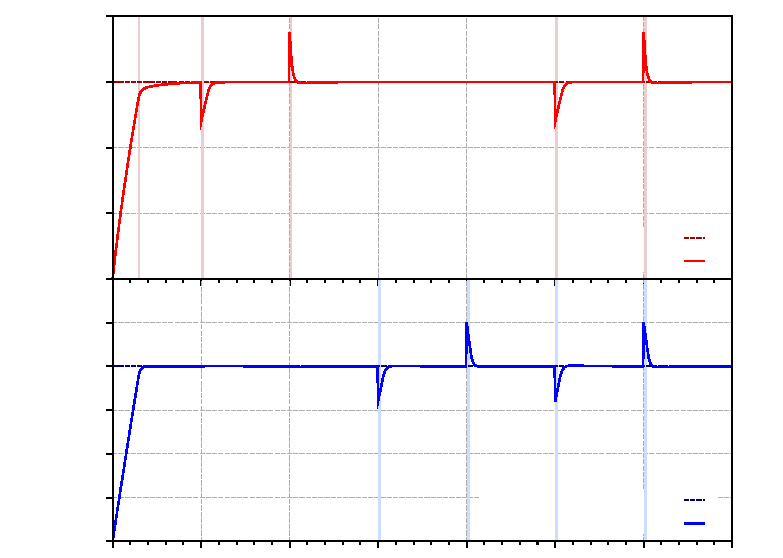
\includegraphics{fsedg}}%
    \gplfronttext
  \end{picture}%
\endgroup

\vspace{1cm}
\caption{Simulação da FSeDG com o ganho reduzido a 80\% do valor original.}
\label{fig:fsedg}
\end{figure}

Observa-se nesta figura que o sistema consegue identificar a presença da falha
assim que o valor do parâmetro é modificado. Após esse período, os controladores
conseguem ``compensar'' a falha, enviando mais tensão para a bomba e,
consequentemente, fazendo com que o nível retorne à referência. Observa-se,
entretanto, que essa ``compensação'' se dá de maneira inadequada, tendo em vista
que a leitura do nível estará com um erro de 20\%. 

Dessa forma, quando o valor lido pelos sensores for de 24\ cm, o tanque estará
prestes a transbordar, atingindo, na verdade, o limite superior de 30\ cm. Em
uma aplicação acadêmica tal situação pode não representar nenhum risco aos
equipamentos além daqueles que a água venha a causar. Por outro lado, em
aplicações críticas essa ``compensação'' pode vir a causar diversos prejuízos.

O sistema se comportou de maneira semelhante na FSeDO e na FSiVzT, conforme
observado nas Figs. \ref{fig:fsedo} e \ref{fig:fsivzt}. Essa semelhança pode vir
a dificultar a identificação dessas falhas quando as redes estiverem agindo
paralelamente. Por outro lado, o sistema composto por uma única rede pode
conseguir diferenciar cada uma dessas falhas de maneira mais eficiente. 

\begin{figure}[htb]
\footnotesize
\centering
% GNUPLOT: LaTeX picture with Postscript
\begingroup
  \makeatletter
  \providecommand\color[2][]{%
    \GenericError{(gnuplot) \space\space\space\@spaces}{%
      Package color not loaded in conjunction with
      terminal option `colourtext'%
    }{See the gnuplot documentation for explanation.%
    }{Either use 'blacktext' in gnuplot or load the package
      color.sty in LaTeX.}%
    \renewcommand\color[2][]{}%
  }%
  \providecommand\includegraphics[2][]{%
    \GenericError{(gnuplot) \space\space\space\@spaces}{%
      Package graphicx or graphics not loaded%
    }{See the gnuplot documentation for explanation.%
    }{The gnuplot epslatex terminal needs graphicx.sty or graphics.sty.}%
    \renewcommand\includegraphics[2][]{}%
  }%
  \providecommand\rotatebox[2]{#2}%
  \@ifundefined{ifGPcolor}{%
    \newif\ifGPcolor
    \GPcolortrue
  }{}%
  \@ifundefined{ifGPblacktext}{%
    \newif\ifGPblacktext
    \GPblacktexttrue
  }{}%
  % define a \g@addto@macro without @ in the name:
  \let\gplgaddtomacro\g@addto@macro
  % define empty templates for all commands taking text:
  \gdef\gplbacktext{}%
  \gdef\gplfronttext{}%
  \makeatother
  \ifGPblacktext
    % no textcolor at all
    \def\colorrgb#1{}%
    \def\colorgray#1{}%
  \else
    % gray or color?
    \ifGPcolor
      \def\colorrgb#1{\color[rgb]{#1}}%
      \def\colorgray#1{\color[gray]{#1}}%
      \expandafter\def\csname LTw\endcsname{\color{white}}%
      \expandafter\def\csname LTb\endcsname{\color{black}}%
      \expandafter\def\csname LTa\endcsname{\color{black}}%
      \expandafter\def\csname LT0\endcsname{\color[rgb]{1,0,0}}%
      \expandafter\def\csname LT1\endcsname{\color[rgb]{0,1,0}}%
      \expandafter\def\csname LT2\endcsname{\color[rgb]{0,0,1}}%
      \expandafter\def\csname LT3\endcsname{\color[rgb]{1,0,1}}%
      \expandafter\def\csname LT4\endcsname{\color[rgb]{0,1,1}}%
      \expandafter\def\csname LT5\endcsname{\color[rgb]{1,1,0}}%
      \expandafter\def\csname LT6\endcsname{\color[rgb]{0,0,0}}%
      \expandafter\def\csname LT7\endcsname{\color[rgb]{1,0.3,0}}%
      \expandafter\def\csname LT8\endcsname{\color[rgb]{0.5,0.5,0.5}}%
    \else
      % gray
      \def\colorrgb#1{\color{black}}%
      \def\colorgray#1{\color[gray]{#1}}%
      \expandafter\def\csname LTw\endcsname{\color{white}}%
      \expandafter\def\csname LTb\endcsname{\color{black}}%
      \expandafter\def\csname LTa\endcsname{\color{black}}%
      \expandafter\def\csname LT0\endcsname{\color{black}}%
      \expandafter\def\csname LT1\endcsname{\color{black}}%
      \expandafter\def\csname LT2\endcsname{\color{black}}%
      \expandafter\def\csname LT3\endcsname{\color{black}}%
      \expandafter\def\csname LT4\endcsname{\color{black}}%
      \expandafter\def\csname LT5\endcsname{\color{black}}%
      \expandafter\def\csname LT6\endcsname{\color{black}}%
      \expandafter\def\csname LT7\endcsname{\color{black}}%
      \expandafter\def\csname LT8\endcsname{\color{black}}%
    \fi
  \fi
  \setlength{\unitlength}{0.0500bp}%
  \begin{picture}(7200.00,5040.00)%
    \gplgaddtomacro\gplbacktext{%
      \csname LTb\endcsname%
      \put(726,3150){\makebox(0,0)[r]{\strut{} 5}}%
      \csname LTb\endcsname%
      \put(726,3780){\makebox(0,0)[r]{\strut{} 10}}%
      \csname LTb\endcsname%
      \put(726,4409){\makebox(0,0)[r]{\strut{} 15}}%
      \csname LTb\endcsname%
      \put(726,5039){\makebox(0,0)[r]{\strut{} 20}}%
      \csname LTb\endcsname%
      \put(921,2237){\makebox(0,0){\strut{}}}%
      \csname LTb\endcsname%
      \put(1771,2237){\makebox(0,0){\strut{}}}%
      \csname LTb\endcsname%
      \put(2620,2237){\makebox(0,0){\strut{}}}%
      \csname LTb\endcsname%
      \put(3470,2237){\makebox(0,0){\strut{}}}%
      \csname LTb\endcsname%
      \put(4320,2237){\makebox(0,0){\strut{}}}%
      \csname LTb\endcsname%
      \put(5170,2237){\makebox(0,0){\strut{}}}%
      \csname LTb\endcsname%
      \put(6019,2237){\makebox(0,0){\strut{}}}%
      \csname LTb\endcsname%
      \put(6869,2237){\makebox(0,0){\strut{}}}%
      \put(352,3779){\rotatebox{-270}{\makebox(0,0){\strut{}Level [cm]}}}%
    }%
    \gplgaddtomacro\gplfronttext{%
      \csname LTb\endcsname%
      \put(6278,2913){\makebox(0,0)[r]{\strut{}Setpoint $T_1$}}%
      \csname LTb\endcsname%
      \put(6278,2693){\makebox(0,0)[r]{\strut{}Output $T_1$}}%
    }%
    \gplgaddtomacro\gplbacktext{%
      \csname LTb\endcsname%
      \put(726,0){\makebox(0,0)[r]{\strut{} 0}}%
      \csname LTb\endcsname%
      \put(726,504){\makebox(0,0)[r]{\strut{} 5}}%
      \csname LTb\endcsname%
      \put(726,1008){\makebox(0,0)[r]{\strut{} 10}}%
      \csname LTb\endcsname%
      \put(726,1512){\makebox(0,0)[r]{\strut{} 15}}%
      \csname LTb\endcsname%
      \put(726,2016){\makebox(0,0)[r]{\strut{} 20}}%
      \csname LTb\endcsname%
      \put(726,2520){\makebox(0,0)[r]{\strut{} 25}}%
      \csname LTb\endcsname%
      \put(921,-283){\makebox(0,0){\strut{}0}}%
      \csname LTb\endcsname%
      \put(1771,-283){\makebox(0,0){\strut{}15}}%
      \csname LTb\endcsname%
      \put(2620,-283){\makebox(0,0){\strut{}30}}%
      \csname LTb\endcsname%
      \put(3470,-283){\makebox(0,0){\strut{}45}}%
      \csname LTb\endcsname%
      \put(4320,-283){\makebox(0,0){\strut{}60}}%
      \csname LTb\endcsname%
      \put(5170,-283){\makebox(0,0){\strut{}75}}%
      \csname LTb\endcsname%
      \put(6019,-283){\makebox(0,0){\strut{}90}}%
      \csname LTb\endcsname%
      \put(6869,-283){\makebox(0,0){\strut{}105}}%
      \put(352,1260){\rotatebox{-270}{\makebox(0,0){\strut{}Level [cm]}}}%
      \put(3895,-613){\makebox(0,0){\strut{}Time [s]}}%
    }%
    \gplgaddtomacro\gplfronttext{%
      \csname LTb\endcsname%
      \put(6278,393){\makebox(0,0)[r]{\strut{}Setpoint $T_2$}}%
      \csname LTb\endcsname%
      \put(6278,173){\makebox(0,0)[r]{\strut{}Output $T_2$}}%
    }%
    \gplbacktext
    \put(0,0){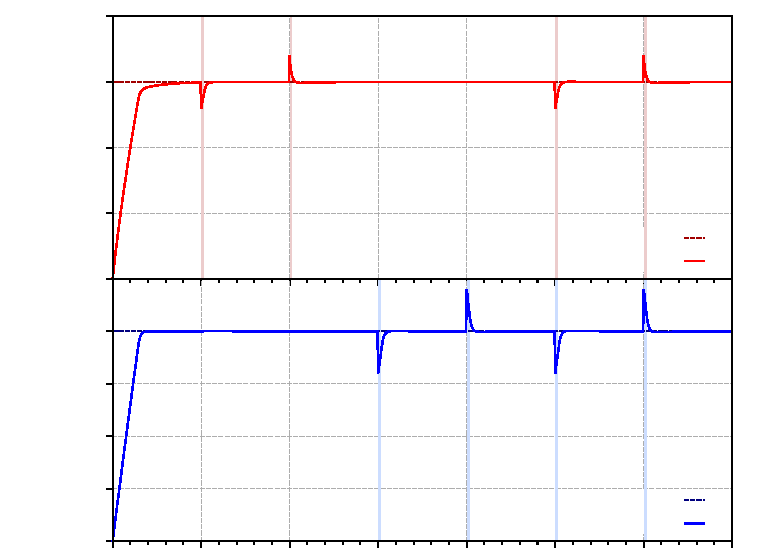
\includegraphics{fsedo}}%
    \gplfronttext
  \end{picture}%
\endgroup

\vspace{1cm}
\caption{Simulação da FSeDO com {\it offset} de -2\ cm.}
\label{fig:fsedo}
\end{figure}

\begin{figure}[htb]
\footnotesize
\centering
% GNUPLOT: LaTeX picture with Postscript
\begingroup
  \makeatletter
  \providecommand\color[2][]{%
    \GenericError{(gnuplot) \space\space\space\@spaces}{%
      Package color not loaded in conjunction with
      terminal option `colourtext'%
    }{See the gnuplot documentation for explanation.%
    }{Either use 'blacktext' in gnuplot or load the package
      color.sty in LaTeX.}%
    \renewcommand\color[2][]{}%
  }%
  \providecommand\includegraphics[2][]{%
    \GenericError{(gnuplot) \space\space\space\@spaces}{%
      Package graphicx or graphics not loaded%
    }{See the gnuplot documentation for explanation.%
    }{The gnuplot epslatex terminal needs graphicx.sty or graphics.sty.}%
    \renewcommand\includegraphics[2][]{}%
  }%
  \providecommand\rotatebox[2]{#2}%
  \@ifundefined{ifGPcolor}{%
    \newif\ifGPcolor
    \GPcolortrue
  }{}%
  \@ifundefined{ifGPblacktext}{%
    \newif\ifGPblacktext
    \GPblacktexttrue
  }{}%
  % define a \g@addto@macro without @ in the name:
  \let\gplgaddtomacro\g@addto@macro
  % define empty templates for all commands taking text:
  \gdef\gplbacktext{}%
  \gdef\gplfronttext{}%
  \makeatother
  \ifGPblacktext
    % no textcolor at all
    \def\colorrgb#1{}%
    \def\colorgray#1{}%
  \else
    % gray or color?
    \ifGPcolor
      \def\colorrgb#1{\color[rgb]{#1}}%
      \def\colorgray#1{\color[gray]{#1}}%
      \expandafter\def\csname LTw\endcsname{\color{white}}%
      \expandafter\def\csname LTb\endcsname{\color{black}}%
      \expandafter\def\csname LTa\endcsname{\color{black}}%
      \expandafter\def\csname LT0\endcsname{\color[rgb]{1,0,0}}%
      \expandafter\def\csname LT1\endcsname{\color[rgb]{0,1,0}}%
      \expandafter\def\csname LT2\endcsname{\color[rgb]{0,0,1}}%
      \expandafter\def\csname LT3\endcsname{\color[rgb]{1,0,1}}%
      \expandafter\def\csname LT4\endcsname{\color[rgb]{0,1,1}}%
      \expandafter\def\csname LT5\endcsname{\color[rgb]{1,1,0}}%
      \expandafter\def\csname LT6\endcsname{\color[rgb]{0,0,0}}%
      \expandafter\def\csname LT7\endcsname{\color[rgb]{1,0.3,0}}%
      \expandafter\def\csname LT8\endcsname{\color[rgb]{0.5,0.5,0.5}}%
    \else
      % gray
      \def\colorrgb#1{\color{black}}%
      \def\colorgray#1{\color[gray]{#1}}%
      \expandafter\def\csname LTw\endcsname{\color{white}}%
      \expandafter\def\csname LTb\endcsname{\color{black}}%
      \expandafter\def\csname LTa\endcsname{\color{black}}%
      \expandafter\def\csname LT0\endcsname{\color{black}}%
      \expandafter\def\csname LT1\endcsname{\color{black}}%
      \expandafter\def\csname LT2\endcsname{\color{black}}%
      \expandafter\def\csname LT3\endcsname{\color{black}}%
      \expandafter\def\csname LT4\endcsname{\color{black}}%
      \expandafter\def\csname LT5\endcsname{\color{black}}%
      \expandafter\def\csname LT6\endcsname{\color{black}}%
      \expandafter\def\csname LT7\endcsname{\color{black}}%
      \expandafter\def\csname LT8\endcsname{\color{black}}%
    \fi
  \fi
  \setlength{\unitlength}{0.0500bp}%
  \begin{picture}(7200.00,5040.00)%
    \gplgaddtomacro\gplbacktext{%
      \csname LTb\endcsname%
      \put(726,3150){\makebox(0,0)[r]{\strut{} 5}}%
      \csname LTb\endcsname%
      \put(726,3780){\makebox(0,0)[r]{\strut{} 10}}%
      \csname LTb\endcsname%
      \put(726,4409){\makebox(0,0)[r]{\strut{} 15}}%
      \csname LTb\endcsname%
      \put(726,5039){\makebox(0,0)[r]{\strut{} 20}}%
      \csname LTb\endcsname%
      \put(921,2237){\makebox(0,0){\strut{}}}%
      \csname LTb\endcsname%
      \put(1771,2237){\makebox(0,0){\strut{}}}%
      \csname LTb\endcsname%
      \put(2620,2237){\makebox(0,0){\strut{}}}%
      \csname LTb\endcsname%
      \put(3470,2237){\makebox(0,0){\strut{}}}%
      \csname LTb\endcsname%
      \put(4320,2237){\makebox(0,0){\strut{}}}%
      \csname LTb\endcsname%
      \put(5170,2237){\makebox(0,0){\strut{}}}%
      \csname LTb\endcsname%
      \put(6019,2237){\makebox(0,0){\strut{}}}%
      \csname LTb\endcsname%
      \put(6869,2237){\makebox(0,0){\strut{}}}%
      \put(352,3779){\rotatebox{-270}{\makebox(0,0){\strut{}Nível [cm]}}}%
    }%
    \gplgaddtomacro\gplfronttext{%
      \csname LTb\endcsname%
      \put(6278,2913){\makebox(0,0)[r]{\strut{}Ref. $T_1$}}%
      \csname LTb\endcsname%
      \put(6278,2693){\makebox(0,0)[r]{\strut{}Saída $T_1$}}%
    }%
    \gplgaddtomacro\gplbacktext{%
      \csname LTb\endcsname%
      \put(726,0){\makebox(0,0)[r]{\strut{} 0}}%
      \csname LTb\endcsname%
      \put(726,840){\makebox(0,0)[r]{\strut{} 10}}%
      \csname LTb\endcsname%
      \put(726,1680){\makebox(0,0)[r]{\strut{} 20}}%
      \csname LTb\endcsname%
      \put(726,2520){\makebox(0,0)[r]{\strut{} 30}}%
      \csname LTb\endcsname%
      \put(921,-283){\makebox(0,0){\strut{}0}}%
      \csname LTb\endcsname%
      \put(1771,-283){\makebox(0,0){\strut{}15}}%
      \csname LTb\endcsname%
      \put(2620,-283){\makebox(0,0){\strut{}30}}%
      \csname LTb\endcsname%
      \put(3470,-283){\makebox(0,0){\strut{}45}}%
      \csname LTb\endcsname%
      \put(4320,-283){\makebox(0,0){\strut{}60}}%
      \csname LTb\endcsname%
      \put(5170,-283){\makebox(0,0){\strut{}75}}%
      \csname LTb\endcsname%
      \put(6019,-283){\makebox(0,0){\strut{}90}}%
      \csname LTb\endcsname%
      \put(6869,-283){\makebox(0,0){\strut{}105}}%
      \put(352,1260){\rotatebox{-270}{\makebox(0,0){\strut{}Nível [cm]}}}%
      \put(3895,-613){\makebox(0,0){\strut{}Tempo [s]}}%
    }%
    \gplgaddtomacro\gplfronttext{%
      \csname LTb\endcsname%
      \put(6278,393){\makebox(0,0)[r]{\strut{}Ref. $T_2$}}%
      \csname LTb\endcsname%
      \put(6278,173){\makebox(0,0)[r]{\strut{}Saída $T_2$}}%
    }%
    \gplbacktext
    \put(0,0){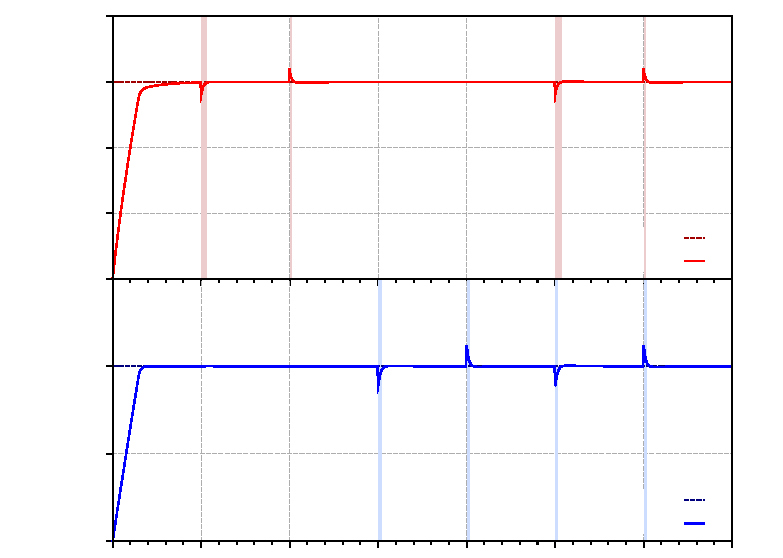
\includegraphics{fsivzt}}%
    \gplfronttext
  \end{picture}%
\endgroup

\vspace{1cm}
\caption{Simulação da FSiVzT com $a_{\tiny VZ} = a_{\tiny MED}/2$.}
\label{fig:fsivzt}
\end{figure}

Os resultados obtidos para essas falhas não estão condizentes com a Tab.
\ref{tab:melhores_redes_detec}. Tal fato pode acontecer porque as redes
identificaram uma dinâmica para variações rápidas através de sinais de excitação
pseudo aleatórios, não conseguindo identificar variações bruscas e continuadas.

Assim, uma possível alternativa para contornar esse problema de detecção, seria
a de se utilizar {\it flags} binárias, ativadas no momento em que fosse
detectada a primeira variação e desativadas na detecção seguinte. Essas {\it
flags} indicariam para o sistema que a falha está agindo durante todo o
intervalo de tempo em que estivessem ativas.

Uma outra simulação mostrou que a FSeSR foi facilmente identificada pelo
sistema, como pode ser visto na Fig. \ref{fig:fsesr}. Observa-se entretanto que,
por se tratar de um ruído com distribuição uniforme ($\pm 2\%$), o sistema não
consegue identificar a falha em alguns pontos. Nesses pontos, pode-se observar
que o valor gerado pela função {\tt rand} mantém o sinal próximo à referência.

\begin{figure}[htb]
\footnotesize
\centering
% GNUPLOT: LaTeX picture with Postscript
\begingroup
  \makeatletter
  \providecommand\color[2][]{%
    \GenericError{(gnuplot) \space\space\space\@spaces}{%
      Package color not loaded in conjunction with
      terminal option `colourtext'%
    }{See the gnuplot documentation for explanation.%
    }{Either use 'blacktext' in gnuplot or load the package
      color.sty in LaTeX.}%
    \renewcommand\color[2][]{}%
  }%
  \providecommand\includegraphics[2][]{%
    \GenericError{(gnuplot) \space\space\space\@spaces}{%
      Package graphicx or graphics not loaded%
    }{See the gnuplot documentation for explanation.%
    }{The gnuplot epslatex terminal needs graphicx.sty or graphics.sty.}%
    \renewcommand\includegraphics[2][]{}%
  }%
  \providecommand\rotatebox[2]{#2}%
  \@ifundefined{ifGPcolor}{%
    \newif\ifGPcolor
    \GPcolortrue
  }{}%
  \@ifundefined{ifGPblacktext}{%
    \newif\ifGPblacktext
    \GPblacktexttrue
  }{}%
  % define a \g@addto@macro without @ in the name:
  \let\gplgaddtomacro\g@addto@macro
  % define empty templates for all commands taking text:
  \gdef\gplbacktext{}%
  \gdef\gplfronttext{}%
  \makeatother
  \ifGPblacktext
    % no textcolor at all
    \def\colorrgb#1{}%
    \def\colorgray#1{}%
  \else
    % gray or color?
    \ifGPcolor
      \def\colorrgb#1{\color[rgb]{#1}}%
      \def\colorgray#1{\color[gray]{#1}}%
      \expandafter\def\csname LTw\endcsname{\color{white}}%
      \expandafter\def\csname LTb\endcsname{\color{black}}%
      \expandafter\def\csname LTa\endcsname{\color{black}}%
      \expandafter\def\csname LT0\endcsname{\color[rgb]{1,0,0}}%
      \expandafter\def\csname LT1\endcsname{\color[rgb]{0,1,0}}%
      \expandafter\def\csname LT2\endcsname{\color[rgb]{0,0,1}}%
      \expandafter\def\csname LT3\endcsname{\color[rgb]{1,0,1}}%
      \expandafter\def\csname LT4\endcsname{\color[rgb]{0,1,1}}%
      \expandafter\def\csname LT5\endcsname{\color[rgb]{1,1,0}}%
      \expandafter\def\csname LT6\endcsname{\color[rgb]{0,0,0}}%
      \expandafter\def\csname LT7\endcsname{\color[rgb]{1,0.3,0}}%
      \expandafter\def\csname LT8\endcsname{\color[rgb]{0.5,0.5,0.5}}%
    \else
      % gray
      \def\colorrgb#1{\color{black}}%
      \def\colorgray#1{\color[gray]{#1}}%
      \expandafter\def\csname LTw\endcsname{\color{white}}%
      \expandafter\def\csname LTb\endcsname{\color{black}}%
      \expandafter\def\csname LTa\endcsname{\color{black}}%
      \expandafter\def\csname LT0\endcsname{\color{black}}%
      \expandafter\def\csname LT1\endcsname{\color{black}}%
      \expandafter\def\csname LT2\endcsname{\color{black}}%
      \expandafter\def\csname LT3\endcsname{\color{black}}%
      \expandafter\def\csname LT4\endcsname{\color{black}}%
      \expandafter\def\csname LT5\endcsname{\color{black}}%
      \expandafter\def\csname LT6\endcsname{\color{black}}%
      \expandafter\def\csname LT7\endcsname{\color{black}}%
      \expandafter\def\csname LT8\endcsname{\color{black}}%
    \fi
  \fi
  \setlength{\unitlength}{0.0500bp}%
  \begin{picture}(7200.00,5040.00)%
    \gplgaddtomacro\gplbacktext{%
      \csname LTb\endcsname%
      \put(726,3150){\makebox(0,0)[r]{\strut{} 5}}%
      \csname LTb\endcsname%
      \put(726,3780){\makebox(0,0)[r]{\strut{} 10}}%
      \csname LTb\endcsname%
      \put(726,4409){\makebox(0,0)[r]{\strut{} 15}}%
      \csname LTb\endcsname%
      \put(726,5039){\makebox(0,0)[r]{\strut{} 20}}%
      \csname LTb\endcsname%
      \put(921,2237){\makebox(0,0){\strut{}}}%
      \csname LTb\endcsname%
      \put(1771,2237){\makebox(0,0){\strut{}}}%
      \csname LTb\endcsname%
      \put(2620,2237){\makebox(0,0){\strut{}}}%
      \csname LTb\endcsname%
      \put(3470,2237){\makebox(0,0){\strut{}}}%
      \csname LTb\endcsname%
      \put(4320,2237){\makebox(0,0){\strut{}}}%
      \csname LTb\endcsname%
      \put(5170,2237){\makebox(0,0){\strut{}}}%
      \csname LTb\endcsname%
      \put(6019,2237){\makebox(0,0){\strut{}}}%
      \csname LTb\endcsname%
      \put(6869,2237){\makebox(0,0){\strut{}}}%
      \put(352,3779){\rotatebox{-270}{\makebox(0,0){\strut{}Nível [cm]}}}%
    }%
    \gplgaddtomacro\gplfronttext{%
      \csname LTb\endcsname%
      \put(6278,2913){\makebox(0,0)[r]{\strut{}Ref. $T_1$}}%
      \csname LTb\endcsname%
      \put(6278,2693){\makebox(0,0)[r]{\strut{}Saída $T_1$}}%
    }%
    \gplgaddtomacro\gplbacktext{%
      \csname LTb\endcsname%
      \put(726,0){\makebox(0,0)[r]{\strut{} 0}}%
      \csname LTb\endcsname%
      \put(726,504){\makebox(0,0)[r]{\strut{} 5}}%
      \csname LTb\endcsname%
      \put(726,1008){\makebox(0,0)[r]{\strut{} 10}}%
      \csname LTb\endcsname%
      \put(726,1512){\makebox(0,0)[r]{\strut{} 15}}%
      \csname LTb\endcsname%
      \put(726,2016){\makebox(0,0)[r]{\strut{} 20}}%
      \csname LTb\endcsname%
      \put(726,2520){\makebox(0,0)[r]{\strut{} 25}}%
      \csname LTb\endcsname%
      \put(921,-283){\makebox(0,0){\strut{}0}}%
      \csname LTb\endcsname%
      \put(1771,-283){\makebox(0,0){\strut{}15}}%
      \csname LTb\endcsname%
      \put(2620,-283){\makebox(0,0){\strut{}30}}%
      \csname LTb\endcsname%
      \put(3470,-283){\makebox(0,0){\strut{}45}}%
      \csname LTb\endcsname%
      \put(4320,-283){\makebox(0,0){\strut{}60}}%
      \csname LTb\endcsname%
      \put(5170,-283){\makebox(0,0){\strut{}75}}%
      \csname LTb\endcsname%
      \put(6019,-283){\makebox(0,0){\strut{}90}}%
      \csname LTb\endcsname%
      \put(6869,-283){\makebox(0,0){\strut{}105}}%
      \put(352,1260){\rotatebox{-270}{\makebox(0,0){\strut{}Nível [cm]}}}%
      \put(3895,-613){\makebox(0,0){\strut{}Tempo [s]}}%
    }%
    \gplgaddtomacro\gplfronttext{%
      \csname LTb\endcsname%
      \put(6278,393){\makebox(0,0)[r]{\strut{}Ref. $T_2$}}%
      \csname LTb\endcsname%
      \put(6278,173){\makebox(0,0)[r]{\strut{}Saída $T_2$}}%
    }%
    \gplbacktext
    \put(0,0){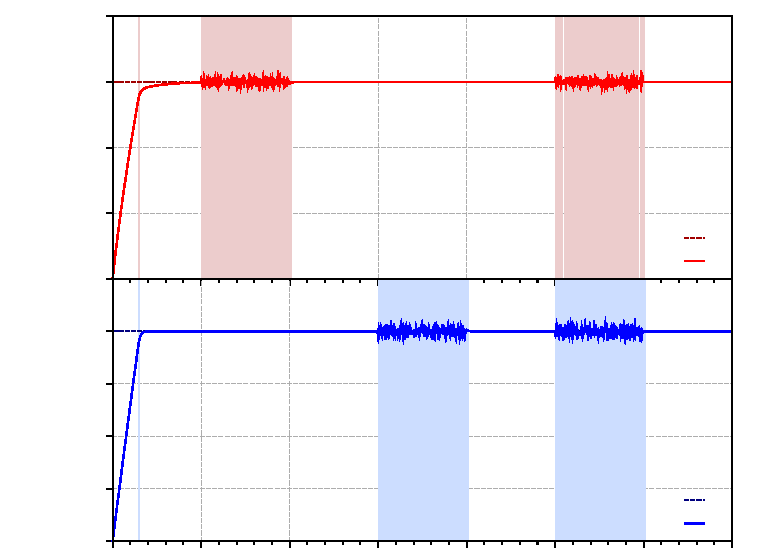
\includegraphics{fsesr}}%
    \gplfronttext
  \end{picture}%
\endgroup

\vspace{1cm}
\caption{Simulação da FSeSR com ruído de distribuição uniforme ($\pm 2\%$).}
\label{fig:fsesr}
\end{figure}

Ao contrário da FSeSR, a FASR entretanto não foi tão facilmente identificada. Os
resultados obtidos para $T_1$ podem até ser considerados razoáveis, contudo, os
resultados para $T_2$ são inaceitáveis, tendo em vista que nenhum dos pontos em
que a falha deveria ter sido identificada foram reconhecidos pela rede. Apesar
disso, observa-se que os resultados estão condizentes com a Tab.
\ref{tab:melhores_redes_detec}, em que o total de erros de detecção supera 40\%.
A simulação da FASR pode ser observada na Fig. \ref{fig:fasr}.

\begin{figure}[htb] \footnotesize \centering % GNUPLOT: LaTeX picture with Postscript
\begingroup
  \makeatletter
  \providecommand\color[2][]{%
    \GenericError{(gnuplot) \space\space\space\@spaces}{%
      Package color not loaded in conjunction with
      terminal option `colourtext'%
    }{See the gnuplot documentation for explanation.%
    }{Either use 'blacktext' in gnuplot or load the package
      color.sty in LaTeX.}%
    \renewcommand\color[2][]{}%
  }%
  \providecommand\includegraphics[2][]{%
    \GenericError{(gnuplot) \space\space\space\@spaces}{%
      Package graphicx or graphics not loaded%
    }{See the gnuplot documentation for explanation.%
    }{The gnuplot epslatex terminal needs graphicx.sty or graphics.sty.}%
    \renewcommand\includegraphics[2][]{}%
  }%
  \providecommand\rotatebox[2]{#2}%
  \@ifundefined{ifGPcolor}{%
    \newif\ifGPcolor
    \GPcolortrue
  }{}%
  \@ifundefined{ifGPblacktext}{%
    \newif\ifGPblacktext
    \GPblacktexttrue
  }{}%
  % define a \g@addto@macro without @ in the name:
  \let\gplgaddtomacro\g@addto@macro
  % define empty templates for all commands taking text:
  \gdef\gplbacktext{}%
  \gdef\gplfronttext{}%
  \makeatother
  \ifGPblacktext
    % no textcolor at all
    \def\colorrgb#1{}%
    \def\colorgray#1{}%
  \else
    % gray or color?
    \ifGPcolor
      \def\colorrgb#1{\color[rgb]{#1}}%
      \def\colorgray#1{\color[gray]{#1}}%
      \expandafter\def\csname LTw\endcsname{\color{white}}%
      \expandafter\def\csname LTb\endcsname{\color{black}}%
      \expandafter\def\csname LTa\endcsname{\color{black}}%
      \expandafter\def\csname LT0\endcsname{\color[rgb]{1,0,0}}%
      \expandafter\def\csname LT1\endcsname{\color[rgb]{0,1,0}}%
      \expandafter\def\csname LT2\endcsname{\color[rgb]{0,0,1}}%
      \expandafter\def\csname LT3\endcsname{\color[rgb]{1,0,1}}%
      \expandafter\def\csname LT4\endcsname{\color[rgb]{0,1,1}}%
      \expandafter\def\csname LT5\endcsname{\color[rgb]{1,1,0}}%
      \expandafter\def\csname LT6\endcsname{\color[rgb]{0,0,0}}%
      \expandafter\def\csname LT7\endcsname{\color[rgb]{1,0.3,0}}%
      \expandafter\def\csname LT8\endcsname{\color[rgb]{0.5,0.5,0.5}}%
    \else
      % gray
      \def\colorrgb#1{\color{black}}%
      \def\colorgray#1{\color[gray]{#1}}%
      \expandafter\def\csname LTw\endcsname{\color{white}}%
      \expandafter\def\csname LTb\endcsname{\color{black}}%
      \expandafter\def\csname LTa\endcsname{\color{black}}%
      \expandafter\def\csname LT0\endcsname{\color{black}}%
      \expandafter\def\csname LT1\endcsname{\color{black}}%
      \expandafter\def\csname LT2\endcsname{\color{black}}%
      \expandafter\def\csname LT3\endcsname{\color{black}}%
      \expandafter\def\csname LT4\endcsname{\color{black}}%
      \expandafter\def\csname LT5\endcsname{\color{black}}%
      \expandafter\def\csname LT6\endcsname{\color{black}}%
      \expandafter\def\csname LT7\endcsname{\color{black}}%
      \expandafter\def\csname LT8\endcsname{\color{black}}%
    \fi
  \fi
  \setlength{\unitlength}{0.0500bp}%
  \begin{picture}(7200.00,5040.00)%
    \gplgaddtomacro\gplbacktext{%
      \csname LTb\endcsname%
      \put(726,3150){\makebox(0,0)[r]{\strut{} 5}}%
      \csname LTb\endcsname%
      \put(726,3780){\makebox(0,0)[r]{\strut{} 10}}%
      \csname LTb\endcsname%
      \put(726,4409){\makebox(0,0)[r]{\strut{} 15}}%
      \csname LTb\endcsname%
      \put(726,5039){\makebox(0,0)[r]{\strut{} 20}}%
      \csname LTb\endcsname%
      \put(921,2237){\makebox(0,0){\strut{}}}%
      \csname LTb\endcsname%
      \put(1771,2237){\makebox(0,0){\strut{}}}%
      \csname LTb\endcsname%
      \put(2620,2237){\makebox(0,0){\strut{}}}%
      \csname LTb\endcsname%
      \put(3470,2237){\makebox(0,0){\strut{}}}%
      \csname LTb\endcsname%
      \put(4320,2237){\makebox(0,0){\strut{}}}%
      \csname LTb\endcsname%
      \put(5170,2237){\makebox(0,0){\strut{}}}%
      \csname LTb\endcsname%
      \put(6019,2237){\makebox(0,0){\strut{}}}%
      \csname LTb\endcsname%
      \put(6869,2237){\makebox(0,0){\strut{}}}%
      \put(352,3779){\rotatebox{-270}{\makebox(0,0){\strut{}Level [cm]}}}%
    }%
    \gplgaddtomacro\gplfronttext{%
      \csname LTb\endcsname%
      \put(6278,2913){\makebox(0,0)[r]{\strut{}Setpoint $T_1$}}%
      \csname LTb\endcsname%
      \put(6278,2693){\makebox(0,0)[r]{\strut{}Output $T_1$}}%
    }%
    \gplgaddtomacro\gplbacktext{%
      \csname LTb\endcsname%
      \put(726,0){\makebox(0,0)[r]{\strut{} 0}}%
      \csname LTb\endcsname%
      \put(726,840){\makebox(0,0)[r]{\strut{} 10}}%
      \csname LTb\endcsname%
      \put(726,1680){\makebox(0,0)[r]{\strut{} 20}}%
      \csname LTb\endcsname%
      \put(726,2520){\makebox(0,0)[r]{\strut{} 30}}%
      \csname LTb\endcsname%
      \put(921,-283){\makebox(0,0){\strut{}0}}%
      \csname LTb\endcsname%
      \put(1771,-283){\makebox(0,0){\strut{}15}}%
      \csname LTb\endcsname%
      \put(2620,-283){\makebox(0,0){\strut{}30}}%
      \csname LTb\endcsname%
      \put(3470,-283){\makebox(0,0){\strut{}45}}%
      \csname LTb\endcsname%
      \put(4320,-283){\makebox(0,0){\strut{}60}}%
      \csname LTb\endcsname%
      \put(5170,-283){\makebox(0,0){\strut{}75}}%
      \csname LTb\endcsname%
      \put(6019,-283){\makebox(0,0){\strut{}90}}%
      \csname LTb\endcsname%
      \put(6869,-283){\makebox(0,0){\strut{}105}}%
      \put(352,1260){\rotatebox{-270}{\makebox(0,0){\strut{}Level [cm]}}}%
      \put(3895,-613){\makebox(0,0){\strut{}Time [s]}}%
    }%
    \gplgaddtomacro\gplfronttext{%
      \csname LTb\endcsname%
      \put(6278,393){\makebox(0,0)[r]{\strut{}Setpoint $T_2$}}%
      \csname LTb\endcsname%
      \put(6278,173){\makebox(0,0)[r]{\strut{}Output $T_2$}}%
    }%
    \gplbacktext
    \put(0,0){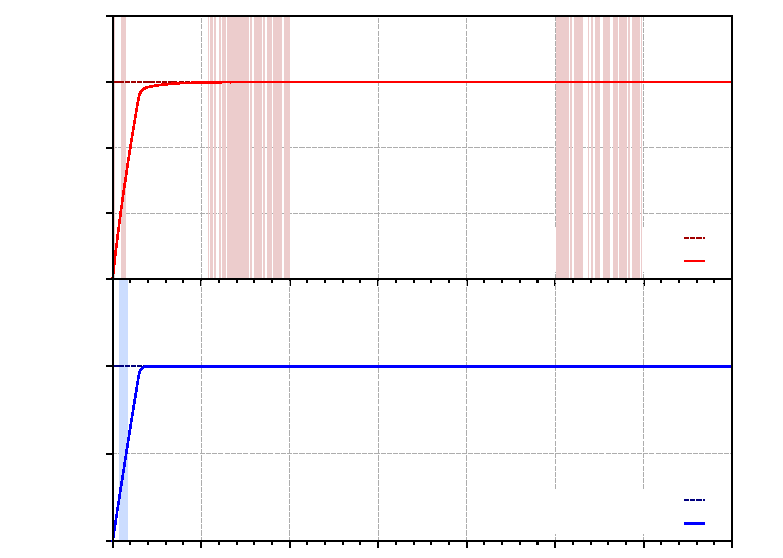
\includegraphics{fasr}}%
    \gplfronttext
  \end{picture}%
\endgroup

\vspace{1cm} \caption{Simulação da FSeSR com ruído de distribuição uniforme
($\pm 2\%$).} \label{fig:fasr} \end{figure}

Com exceção da FSiVrGMP, todas as falhas restantes também foram facilmente
identificadas pelo sistema, como pode ser observado nas Figs. \ref{fig:fseq} a
\ref{fig:fsieos}. No caso da FSiVrGMP, o sistema não consegue detectar quando a
falha acontece somente em $T_1$, como pode ser visto no intervalo de 15 (quinze)
a 30 (trinta) segundos da Fig. \ref{fig:fsivrgmp}. Todavia, as falhas em $T_2$
são identificadas corretamente. Tal fato justifica a quantidade de erros
expostos pela Tab. \ref{tab:melhores_redes_detec}.

\begin{figure}[htb]
\footnotesize
\centering
% GNUPLOT: LaTeX picture with Postscript
\begingroup
  \makeatletter
  \providecommand\color[2][]{%
    \GenericError{(gnuplot) \space\space\space\@spaces}{%
      Package color not loaded in conjunction with
      terminal option `colourtext'%
    }{See the gnuplot documentation for explanation.%
    }{Either use 'blacktext' in gnuplot or load the package
      color.sty in LaTeX.}%
    \renewcommand\color[2][]{}%
  }%
  \providecommand\includegraphics[2][]{%
    \GenericError{(gnuplot) \space\space\space\@spaces}{%
      Package graphicx or graphics not loaded%
    }{See the gnuplot documentation for explanation.%
    }{The gnuplot epslatex terminal needs graphicx.sty or graphics.sty.}%
    \renewcommand\includegraphics[2][]{}%
  }%
  \providecommand\rotatebox[2]{#2}%
  \@ifundefined{ifGPcolor}{%
    \newif\ifGPcolor
    \GPcolortrue
  }{}%
  \@ifundefined{ifGPblacktext}{%
    \newif\ifGPblacktext
    \GPblacktexttrue
  }{}%
  % define a \g@addto@macro without @ in the name:
  \let\gplgaddtomacro\g@addto@macro
  % define empty templates for all commands taking text:
  \gdef\gplbacktext{}%
  \gdef\gplfronttext{}%
  \makeatother
  \ifGPblacktext
    % no textcolor at all
    \def\colorrgb#1{}%
    \def\colorgray#1{}%
  \else
    % gray or color?
    \ifGPcolor
      \def\colorrgb#1{\color[rgb]{#1}}%
      \def\colorgray#1{\color[gray]{#1}}%
      \expandafter\def\csname LTw\endcsname{\color{white}}%
      \expandafter\def\csname LTb\endcsname{\color{black}}%
      \expandafter\def\csname LTa\endcsname{\color{black}}%
      \expandafter\def\csname LT0\endcsname{\color[rgb]{1,0,0}}%
      \expandafter\def\csname LT1\endcsname{\color[rgb]{0,1,0}}%
      \expandafter\def\csname LT2\endcsname{\color[rgb]{0,0,1}}%
      \expandafter\def\csname LT3\endcsname{\color[rgb]{1,0,1}}%
      \expandafter\def\csname LT4\endcsname{\color[rgb]{0,1,1}}%
      \expandafter\def\csname LT5\endcsname{\color[rgb]{1,1,0}}%
      \expandafter\def\csname LT6\endcsname{\color[rgb]{0,0,0}}%
      \expandafter\def\csname LT7\endcsname{\color[rgb]{1,0.3,0}}%
      \expandafter\def\csname LT8\endcsname{\color[rgb]{0.5,0.5,0.5}}%
    \else
      % gray
      \def\colorrgb#1{\color{black}}%
      \def\colorgray#1{\color[gray]{#1}}%
      \expandafter\def\csname LTw\endcsname{\color{white}}%
      \expandafter\def\csname LTb\endcsname{\color{black}}%
      \expandafter\def\csname LTa\endcsname{\color{black}}%
      \expandafter\def\csname LT0\endcsname{\color{black}}%
      \expandafter\def\csname LT1\endcsname{\color{black}}%
      \expandafter\def\csname LT2\endcsname{\color{black}}%
      \expandafter\def\csname LT3\endcsname{\color{black}}%
      \expandafter\def\csname LT4\endcsname{\color{black}}%
      \expandafter\def\csname LT5\endcsname{\color{black}}%
      \expandafter\def\csname LT6\endcsname{\color{black}}%
      \expandafter\def\csname LT7\endcsname{\color{black}}%
      \expandafter\def\csname LT8\endcsname{\color{black}}%
    \fi
  \fi
  \setlength{\unitlength}{0.0500bp}%
  \begin{picture}(7200.00,5040.00)%
    \gplgaddtomacro\gplbacktext{%
      \csname LTb\endcsname%
      \put(726,3150){\makebox(0,0)[r]{\strut{} 5}}%
      \csname LTb\endcsname%
      \put(726,3780){\makebox(0,0)[r]{\strut{} 10}}%
      \csname LTb\endcsname%
      \put(726,4409){\makebox(0,0)[r]{\strut{} 15}}%
      \csname LTb\endcsname%
      \put(726,5039){\makebox(0,0)[r]{\strut{} 20}}%
      \csname LTb\endcsname%
      \put(921,2237){\makebox(0,0){\strut{}}}%
      \csname LTb\endcsname%
      \put(1771,2237){\makebox(0,0){\strut{}}}%
      \csname LTb\endcsname%
      \put(2620,2237){\makebox(0,0){\strut{}}}%
      \csname LTb\endcsname%
      \put(3470,2237){\makebox(0,0){\strut{}}}%
      \csname LTb\endcsname%
      \put(4320,2237){\makebox(0,0){\strut{}}}%
      \csname LTb\endcsname%
      \put(5170,2237){\makebox(0,0){\strut{}}}%
      \csname LTb\endcsname%
      \put(6019,2237){\makebox(0,0){\strut{}}}%
      \csname LTb\endcsname%
      \put(6869,2237){\makebox(0,0){\strut{}}}%
      \put(352,3779){\rotatebox{-270}{\makebox(0,0){\strut{}Nível [cm]}}}%
    }%
    \gplgaddtomacro\gplfronttext{%
      \csname LTb\endcsname%
      \put(6278,2913){\makebox(0,0)[r]{\strut{}Ref. $T_1$}}%
      \csname LTb\endcsname%
      \put(6278,2693){\makebox(0,0)[r]{\strut{}Saída $T_1$}}%
    }%
    \gplgaddtomacro\gplbacktext{%
      \csname LTb\endcsname%
      \put(726,0){\makebox(0,0)[r]{\strut{} 0}}%
      \csname LTb\endcsname%
      \put(726,840){\makebox(0,0)[r]{\strut{} 10}}%
      \csname LTb\endcsname%
      \put(726,1680){\makebox(0,0)[r]{\strut{} 20}}%
      \csname LTb\endcsname%
      \put(726,2520){\makebox(0,0)[r]{\strut{} 30}}%
      \csname LTb\endcsname%
      \put(921,-283){\makebox(0,0){\strut{}0}}%
      \csname LTb\endcsname%
      \put(1771,-283){\makebox(0,0){\strut{}15}}%
      \csname LTb\endcsname%
      \put(2620,-283){\makebox(0,0){\strut{}30}}%
      \csname LTb\endcsname%
      \put(3470,-283){\makebox(0,0){\strut{}45}}%
      \csname LTb\endcsname%
      \put(4320,-283){\makebox(0,0){\strut{}60}}%
      \csname LTb\endcsname%
      \put(5170,-283){\makebox(0,0){\strut{}75}}%
      \csname LTb\endcsname%
      \put(6019,-283){\makebox(0,0){\strut{}90}}%
      \csname LTb\endcsname%
      \put(6869,-283){\makebox(0,0){\strut{}105}}%
      \put(352,1260){\rotatebox{-270}{\makebox(0,0){\strut{}Nível [cm]}}}%
      \put(3895,-613){\makebox(0,0){\strut{}Tempo [s]}}%
    }%
    \gplgaddtomacro\gplfronttext{%
      \csname LTb\endcsname%
      \put(6278,393){\makebox(0,0)[r]{\strut{}Ref. $T_2$}}%
      \csname LTb\endcsname%
      \put(6278,173){\makebox(0,0)[r]{\strut{}Saída $T_2$}}%
    }%
    \gplbacktext
    \put(0,0){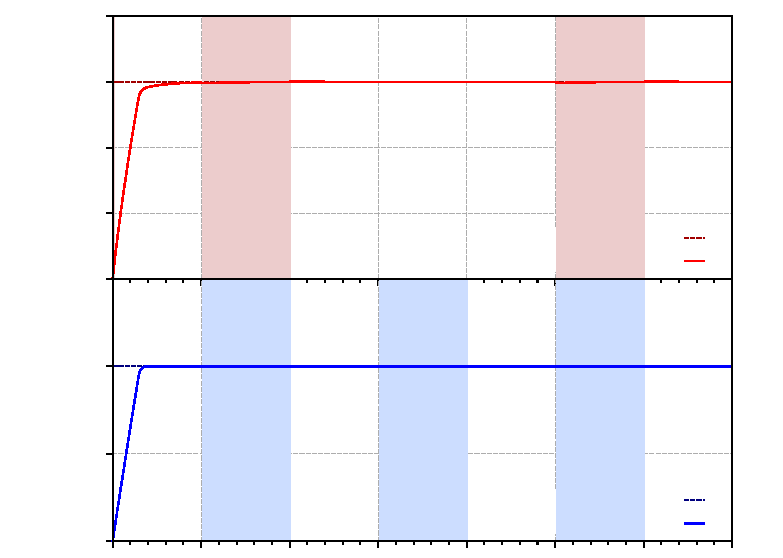
\includegraphics{fsivrgmp}}%
    \gplfronttext
  \end{picture}%
\endgroup

\vspace{1cm}
\caption{Simulação da FSiVrGMP com o ganho reduzido a 90\% do valor original.}
\label{fig:fsivrgmp}
\end{figure}

\begin{figure}[htb]
\footnotesize
\centering
% GNUPLOT: LaTeX picture with Postscript
\begingroup
  \makeatletter
  \providecommand\color[2][]{%
    \GenericError{(gnuplot) \space\space\space\@spaces}{%
      Package color not loaded in conjunction with
      terminal option `colourtext'%
    }{See the gnuplot documentation for explanation.%
    }{Either use 'blacktext' in gnuplot or load the package
      color.sty in LaTeX.}%
    \renewcommand\color[2][]{}%
  }%
  \providecommand\includegraphics[2][]{%
    \GenericError{(gnuplot) \space\space\space\@spaces}{%
      Package graphicx or graphics not loaded%
    }{See the gnuplot documentation for explanation.%
    }{The gnuplot epslatex terminal needs graphicx.sty or graphics.sty.}%
    \renewcommand\includegraphics[2][]{}%
  }%
  \providecommand\rotatebox[2]{#2}%
  \@ifundefined{ifGPcolor}{%
    \newif\ifGPcolor
    \GPcolortrue
  }{}%
  \@ifundefined{ifGPblacktext}{%
    \newif\ifGPblacktext
    \GPblacktexttrue
  }{}%
  % define a \g@addto@macro without @ in the name:
  \let\gplgaddtomacro\g@addto@macro
  % define empty templates for all commands taking text:
  \gdef\gplbacktext{}%
  \gdef\gplfronttext{}%
  \makeatother
  \ifGPblacktext
    % no textcolor at all
    \def\colorrgb#1{}%
    \def\colorgray#1{}%
  \else
    % gray or color?
    \ifGPcolor
      \def\colorrgb#1{\color[rgb]{#1}}%
      \def\colorgray#1{\color[gray]{#1}}%
      \expandafter\def\csname LTw\endcsname{\color{white}}%
      \expandafter\def\csname LTb\endcsname{\color{black}}%
      \expandafter\def\csname LTa\endcsname{\color{black}}%
      \expandafter\def\csname LT0\endcsname{\color[rgb]{1,0,0}}%
      \expandafter\def\csname LT1\endcsname{\color[rgb]{0,1,0}}%
      \expandafter\def\csname LT2\endcsname{\color[rgb]{0,0,1}}%
      \expandafter\def\csname LT3\endcsname{\color[rgb]{1,0,1}}%
      \expandafter\def\csname LT4\endcsname{\color[rgb]{0,1,1}}%
      \expandafter\def\csname LT5\endcsname{\color[rgb]{1,1,0}}%
      \expandafter\def\csname LT6\endcsname{\color[rgb]{0,0,0}}%
      \expandafter\def\csname LT7\endcsname{\color[rgb]{1,0.3,0}}%
      \expandafter\def\csname LT8\endcsname{\color[rgb]{0.5,0.5,0.5}}%
    \else
      % gray
      \def\colorrgb#1{\color{black}}%
      \def\colorgray#1{\color[gray]{#1}}%
      \expandafter\def\csname LTw\endcsname{\color{white}}%
      \expandafter\def\csname LTb\endcsname{\color{black}}%
      \expandafter\def\csname LTa\endcsname{\color{black}}%
      \expandafter\def\csname LT0\endcsname{\color{black}}%
      \expandafter\def\csname LT1\endcsname{\color{black}}%
      \expandafter\def\csname LT2\endcsname{\color{black}}%
      \expandafter\def\csname LT3\endcsname{\color{black}}%
      \expandafter\def\csname LT4\endcsname{\color{black}}%
      \expandafter\def\csname LT5\endcsname{\color{black}}%
      \expandafter\def\csname LT6\endcsname{\color{black}}%
      \expandafter\def\csname LT7\endcsname{\color{black}}%
      \expandafter\def\csname LT8\endcsname{\color{black}}%
    \fi
  \fi
  \setlength{\unitlength}{0.0500bp}%
  \begin{picture}(7200.00,5040.00)%
    \gplgaddtomacro\gplbacktext{%
      \csname LTb\endcsname%
      \put(726,2800){\makebox(0,0)[r]{\strut{} 5}}%
      \csname LTb\endcsname%
      \put(726,3080){\makebox(0,0)[r]{\strut{} 10}}%
      \csname LTb\endcsname%
      \put(726,3360){\makebox(0,0)[r]{\strut{} 15}}%
      \csname LTb\endcsname%
      \put(726,3640){\makebox(0,0)[r]{\strut{} 20}}%
      \csname LTb\endcsname%
      \put(726,3919){\makebox(0,0)[r]{\strut{} 25}}%
      \csname LTb\endcsname%
      \put(726,4199){\makebox(0,0)[r]{\strut{} 30}}%
      \csname LTb\endcsname%
      \put(726,4479){\makebox(0,0)[r]{\strut{} 35}}%
      \csname LTb\endcsname%
      \put(726,4759){\makebox(0,0)[r]{\strut{} 40}}%
      \csname LTb\endcsname%
      \put(726,5039){\makebox(0,0)[r]{\strut{} 45}}%
      \csname LTb\endcsname%
      \put(921,2237){\makebox(0,0){\strut{}}}%
      \csname LTb\endcsname%
      \put(1771,2237){\makebox(0,0){\strut{}}}%
      \csname LTb\endcsname%
      \put(2620,2237){\makebox(0,0){\strut{}}}%
      \csname LTb\endcsname%
      \put(3470,2237){\makebox(0,0){\strut{}}}%
      \csname LTb\endcsname%
      \put(4320,2237){\makebox(0,0){\strut{}}}%
      \csname LTb\endcsname%
      \put(5170,2237){\makebox(0,0){\strut{}}}%
      \csname LTb\endcsname%
      \put(6019,2237){\makebox(0,0){\strut{}}}%
      \csname LTb\endcsname%
      \put(6869,2237){\makebox(0,0){\strut{}}}%
      \put(352,3779){\rotatebox{-270}{\makebox(0,0){\strut{}Level [cm]}}}%
    }%
    \gplgaddtomacro\gplfronttext{%
      \csname LTb\endcsname%
      \put(6278,2913){\makebox(0,0)[r]{\strut{}Setpoint $T_1$}}%
      \csname LTb\endcsname%
      \put(6278,2693){\makebox(0,0)[r]{\strut{}Output $T_1$}}%
    }%
    \gplgaddtomacro\gplbacktext{%
      \csname LTb\endcsname%
      \put(726,0){\makebox(0,0)[r]{\strut{} 0}}%
      \csname LTb\endcsname%
      \put(726,315){\makebox(0,0)[r]{\strut{} 10}}%
      \csname LTb\endcsname%
      \put(726,630){\makebox(0,0)[r]{\strut{} 20}}%
      \csname LTb\endcsname%
      \put(726,945){\makebox(0,0)[r]{\strut{} 30}}%
      \csname LTb\endcsname%
      \put(726,1260){\makebox(0,0)[r]{\strut{} 40}}%
      \csname LTb\endcsname%
      \put(726,1575){\makebox(0,0)[r]{\strut{} 50}}%
      \csname LTb\endcsname%
      \put(726,1890){\makebox(0,0)[r]{\strut{} 60}}%
      \csname LTb\endcsname%
      \put(726,2205){\makebox(0,0)[r]{\strut{} 70}}%
      \csname LTb\endcsname%
      \put(726,2520){\makebox(0,0)[r]{\strut{} 80}}%
      \csname LTb\endcsname%
      \put(921,-283){\makebox(0,0){\strut{}0}}%
      \csname LTb\endcsname%
      \put(1771,-283){\makebox(0,0){\strut{}15}}%
      \csname LTb\endcsname%
      \put(2620,-283){\makebox(0,0){\strut{}30}}%
      \csname LTb\endcsname%
      \put(3470,-283){\makebox(0,0){\strut{}45}}%
      \csname LTb\endcsname%
      \put(4320,-283){\makebox(0,0){\strut{}60}}%
      \csname LTb\endcsname%
      \put(5170,-283){\makebox(0,0){\strut{}75}}%
      \csname LTb\endcsname%
      \put(6019,-283){\makebox(0,0){\strut{}90}}%
      \csname LTb\endcsname%
      \put(6869,-283){\makebox(0,0){\strut{}105}}%
      \put(352,1260){\rotatebox{-270}{\makebox(0,0){\strut{}Level [cm]}}}%
      \put(3895,-613){\makebox(0,0){\strut{}Time [s]}}%
    }%
    \gplgaddtomacro\gplfronttext{%
      \csname LTb\endcsname%
      \put(6278,393){\makebox(0,0)[r]{\strut{}Setpoint $T_2$}}%
      \csname LTb\endcsname%
      \put(6278,173){\makebox(0,0)[r]{\strut{}Output $T_2$}}%
    }%
    \gplbacktext
    \put(0,0){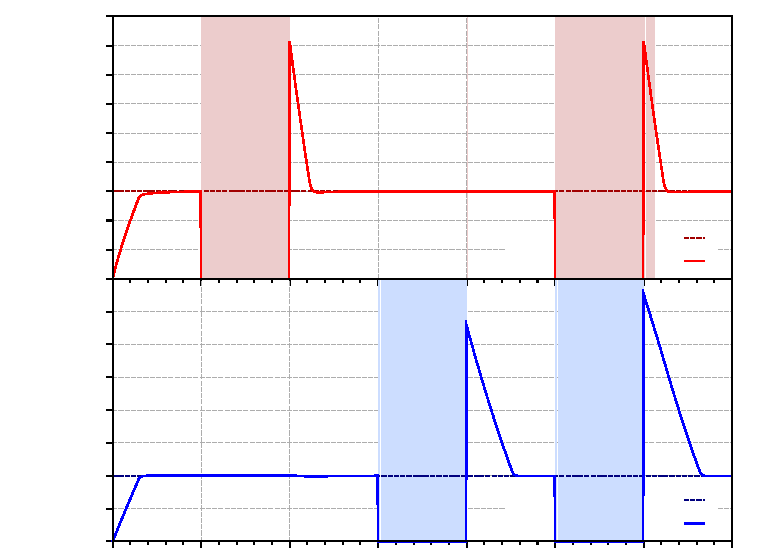
\includegraphics{fseq}}%
    \gplfronttext
  \end{picture}%
\endgroup

\vspace{1cm}
\caption{Simulação da FSeQ (Ganho = 0).}
\label{fig:fseq}
\end{figure}

\begin{figure}[htb]
\footnotesize
\centering
% GNUPLOT: LaTeX picture with Postscript
\begingroup
  \makeatletter
  \providecommand\color[2][]{%
    \GenericError{(gnuplot) \space\space\space\@spaces}{%
      Package color not loaded in conjunction with
      terminal option `colourtext'%
    }{See the gnuplot documentation for explanation.%
    }{Either use 'blacktext' in gnuplot or load the package
      color.sty in LaTeX.}%
    \renewcommand\color[2][]{}%
  }%
  \providecommand\includegraphics[2][]{%
    \GenericError{(gnuplot) \space\space\space\@spaces}{%
      Package graphicx or graphics not loaded%
    }{See the gnuplot documentation for explanation.%
    }{The gnuplot epslatex terminal needs graphicx.sty or graphics.sty.}%
    \renewcommand\includegraphics[2][]{}%
  }%
  \providecommand\rotatebox[2]{#2}%
  \@ifundefined{ifGPcolor}{%
    \newif\ifGPcolor
    \GPcolortrue
  }{}%
  \@ifundefined{ifGPblacktext}{%
    \newif\ifGPblacktext
    \GPblacktexttrue
  }{}%
  % define a \g@addto@macro without @ in the name:
  \let\gplgaddtomacro\g@addto@macro
  % define empty templates for all commands taking text:
  \gdef\gplbacktext{}%
  \gdef\gplfronttext{}%
  \makeatother
  \ifGPblacktext
    % no textcolor at all
    \def\colorrgb#1{}%
    \def\colorgray#1{}%
  \else
    % gray or color?
    \ifGPcolor
      \def\colorrgb#1{\color[rgb]{#1}}%
      \def\colorgray#1{\color[gray]{#1}}%
      \expandafter\def\csname LTw\endcsname{\color{white}}%
      \expandafter\def\csname LTb\endcsname{\color{black}}%
      \expandafter\def\csname LTa\endcsname{\color{black}}%
      \expandafter\def\csname LT0\endcsname{\color[rgb]{1,0,0}}%
      \expandafter\def\csname LT1\endcsname{\color[rgb]{0,1,0}}%
      \expandafter\def\csname LT2\endcsname{\color[rgb]{0,0,1}}%
      \expandafter\def\csname LT3\endcsname{\color[rgb]{1,0,1}}%
      \expandafter\def\csname LT4\endcsname{\color[rgb]{0,1,1}}%
      \expandafter\def\csname LT5\endcsname{\color[rgb]{1,1,0}}%
      \expandafter\def\csname LT6\endcsname{\color[rgb]{0,0,0}}%
      \expandafter\def\csname LT7\endcsname{\color[rgb]{1,0.3,0}}%
      \expandafter\def\csname LT8\endcsname{\color[rgb]{0.5,0.5,0.5}}%
    \else
      % gray
      \def\colorrgb#1{\color{black}}%
      \def\colorgray#1{\color[gray]{#1}}%
      \expandafter\def\csname LTw\endcsname{\color{white}}%
      \expandafter\def\csname LTb\endcsname{\color{black}}%
      \expandafter\def\csname LTa\endcsname{\color{black}}%
      \expandafter\def\csname LT0\endcsname{\color{black}}%
      \expandafter\def\csname LT1\endcsname{\color{black}}%
      \expandafter\def\csname LT2\endcsname{\color{black}}%
      \expandafter\def\csname LT3\endcsname{\color{black}}%
      \expandafter\def\csname LT4\endcsname{\color{black}}%
      \expandafter\def\csname LT5\endcsname{\color{black}}%
      \expandafter\def\csname LT6\endcsname{\color{black}}%
      \expandafter\def\csname LT7\endcsname{\color{black}}%
      \expandafter\def\csname LT8\endcsname{\color{black}}%
    \fi
  \fi
  \setlength{\unitlength}{0.0500bp}%
  \begin{picture}(7200.00,5040.00)%
    \gplgaddtomacro\gplbacktext{%
      \csname LTb\endcsname%
      \put(726,3150){\makebox(0,0)[r]{\strut{} 5}}%
      \csname LTb\endcsname%
      \put(726,3780){\makebox(0,0)[r]{\strut{} 10}}%
      \csname LTb\endcsname%
      \put(726,4409){\makebox(0,0)[r]{\strut{} 15}}%
      \csname LTb\endcsname%
      \put(726,5039){\makebox(0,0)[r]{\strut{} 20}}%
      \csname LTb\endcsname%
      \put(921,2237){\makebox(0,0){\strut{}}}%
      \csname LTb\endcsname%
      \put(1771,2237){\makebox(0,0){\strut{}}}%
      \csname LTb\endcsname%
      \put(2620,2237){\makebox(0,0){\strut{}}}%
      \csname LTb\endcsname%
      \put(3470,2237){\makebox(0,0){\strut{}}}%
      \csname LTb\endcsname%
      \put(4320,2237){\makebox(0,0){\strut{}}}%
      \csname LTb\endcsname%
      \put(5170,2237){\makebox(0,0){\strut{}}}%
      \csname LTb\endcsname%
      \put(6019,2237){\makebox(0,0){\strut{}}}%
      \csname LTb\endcsname%
      \put(6869,2237){\makebox(0,0){\strut{}}}%
      \put(352,3779){\rotatebox{-270}{\makebox(0,0){\strut{}Nível [cm]}}}%
    }%
    \gplgaddtomacro\gplfronttext{%
      \csname LTb\endcsname%
      \put(6278,2913){\makebox(0,0)[r]{\strut{}Ref. $T_1$}}%
      \csname LTb\endcsname%
      \put(6278,2693){\makebox(0,0)[r]{\strut{}Saída $T_1$}}%
    }%
    \gplgaddtomacro\gplbacktext{%
      \csname LTb\endcsname%
      \put(726,0){\makebox(0,0)[r]{\strut{} 0}}%
      \csname LTb\endcsname%
      \put(726,840){\makebox(0,0)[r]{\strut{} 10}}%
      \csname LTb\endcsname%
      \put(726,1680){\makebox(0,0)[r]{\strut{} 20}}%
      \csname LTb\endcsname%
      \put(726,2520){\makebox(0,0)[r]{\strut{} 30}}%
      \csname LTb\endcsname%
      \put(921,-283){\makebox(0,0){\strut{}0}}%
      \csname LTb\endcsname%
      \put(1771,-283){\makebox(0,0){\strut{}15}}%
      \csname LTb\endcsname%
      \put(2620,-283){\makebox(0,0){\strut{}30}}%
      \csname LTb\endcsname%
      \put(3470,-283){\makebox(0,0){\strut{}45}}%
      \csname LTb\endcsname%
      \put(4320,-283){\makebox(0,0){\strut{}60}}%
      \csname LTb\endcsname%
      \put(5170,-283){\makebox(0,0){\strut{}75}}%
      \csname LTb\endcsname%
      \put(6019,-283){\makebox(0,0){\strut{}90}}%
      \csname LTb\endcsname%
      \put(6869,-283){\makebox(0,0){\strut{}105}}%
      \put(352,1260){\rotatebox{-270}{\makebox(0,0){\strut{}Nível [cm]}}}%
      \put(3895,-613){\makebox(0,0){\strut{}Tempo [s]}}%
    }%
    \gplgaddtomacro\gplfronttext{%
      \csname LTb\endcsname%
      \put(6278,393){\makebox(0,0)[r]{\strut{}Ref. $T_2$}}%
      \csname LTb\endcsname%
      \put(6278,173){\makebox(0,0)[r]{\strut{}Saída $T_2$}}%
    }%
    \gplbacktext
    \put(0,0){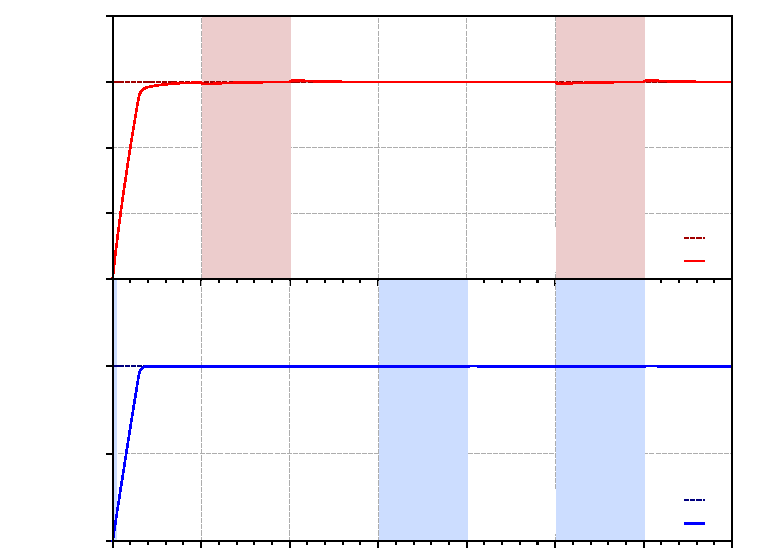
\includegraphics{fadg}}%
    \gplfronttext
  \end{picture}%
\endgroup

\vspace{1cm}
\caption{Simulação da FADG com o ganho reduzido a 80\% do valor original.}
\label{fig:fadg}
\end{figure}

\begin{figure}[htb]
\footnotesize
\centering
% GNUPLOT: LaTeX picture with Postscript
\begingroup
  \makeatletter
  \providecommand\color[2][]{%
    \GenericError{(gnuplot) \space\space\space\@spaces}{%
      Package color not loaded in conjunction with
      terminal option `colourtext'%
    }{See the gnuplot documentation for explanation.%
    }{Either use 'blacktext' in gnuplot or load the package
      color.sty in LaTeX.}%
    \renewcommand\color[2][]{}%
  }%
  \providecommand\includegraphics[2][]{%
    \GenericError{(gnuplot) \space\space\space\@spaces}{%
      Package graphicx or graphics not loaded%
    }{See the gnuplot documentation for explanation.%
    }{The gnuplot epslatex terminal needs graphicx.sty or graphics.sty.}%
    \renewcommand\includegraphics[2][]{}%
  }%
  \providecommand\rotatebox[2]{#2}%
  \@ifundefined{ifGPcolor}{%
    \newif\ifGPcolor
    \GPcolortrue
  }{}%
  \@ifundefined{ifGPblacktext}{%
    \newif\ifGPblacktext
    \GPblacktexttrue
  }{}%
  % define a \g@addto@macro without @ in the name:
  \let\gplgaddtomacro\g@addto@macro
  % define empty templates for all commands taking text:
  \gdef\gplbacktext{}%
  \gdef\gplfronttext{}%
  \makeatother
  \ifGPblacktext
    % no textcolor at all
    \def\colorrgb#1{}%
    \def\colorgray#1{}%
  \else
    % gray or color?
    \ifGPcolor
      \def\colorrgb#1{\color[rgb]{#1}}%
      \def\colorgray#1{\color[gray]{#1}}%
      \expandafter\def\csname LTw\endcsname{\color{white}}%
      \expandafter\def\csname LTb\endcsname{\color{black}}%
      \expandafter\def\csname LTa\endcsname{\color{black}}%
      \expandafter\def\csname LT0\endcsname{\color[rgb]{1,0,0}}%
      \expandafter\def\csname LT1\endcsname{\color[rgb]{0,1,0}}%
      \expandafter\def\csname LT2\endcsname{\color[rgb]{0,0,1}}%
      \expandafter\def\csname LT3\endcsname{\color[rgb]{1,0,1}}%
      \expandafter\def\csname LT4\endcsname{\color[rgb]{0,1,1}}%
      \expandafter\def\csname LT5\endcsname{\color[rgb]{1,1,0}}%
      \expandafter\def\csname LT6\endcsname{\color[rgb]{0,0,0}}%
      \expandafter\def\csname LT7\endcsname{\color[rgb]{1,0.3,0}}%
      \expandafter\def\csname LT8\endcsname{\color[rgb]{0.5,0.5,0.5}}%
    \else
      % gray
      \def\colorrgb#1{\color{black}}%
      \def\colorgray#1{\color[gray]{#1}}%
      \expandafter\def\csname LTw\endcsname{\color{white}}%
      \expandafter\def\csname LTb\endcsname{\color{black}}%
      \expandafter\def\csname LTa\endcsname{\color{black}}%
      \expandafter\def\csname LT0\endcsname{\color{black}}%
      \expandafter\def\csname LT1\endcsname{\color{black}}%
      \expandafter\def\csname LT2\endcsname{\color{black}}%
      \expandafter\def\csname LT3\endcsname{\color{black}}%
      \expandafter\def\csname LT4\endcsname{\color{black}}%
      \expandafter\def\csname LT5\endcsname{\color{black}}%
      \expandafter\def\csname LT6\endcsname{\color{black}}%
      \expandafter\def\csname LT7\endcsname{\color{black}}%
      \expandafter\def\csname LT8\endcsname{\color{black}}%
    \fi
  \fi
  \setlength{\unitlength}{0.0500bp}%
  \begin{picture}(7200.00,5040.00)%
    \gplgaddtomacro\gplbacktext{%
      \csname LTb\endcsname%
      \put(726,3150){\makebox(0,0)[r]{\strut{} 5}}%
      \csname LTb\endcsname%
      \put(726,3780){\makebox(0,0)[r]{\strut{} 10}}%
      \csname LTb\endcsname%
      \put(726,4409){\makebox(0,0)[r]{\strut{} 15}}%
      \csname LTb\endcsname%
      \put(726,5039){\makebox(0,0)[r]{\strut{} 20}}%
      \csname LTb\endcsname%
      \put(921,2237){\makebox(0,0){\strut{}}}%
      \csname LTb\endcsname%
      \put(1771,2237){\makebox(0,0){\strut{}}}%
      \csname LTb\endcsname%
      \put(2620,2237){\makebox(0,0){\strut{}}}%
      \csname LTb\endcsname%
      \put(3470,2237){\makebox(0,0){\strut{}}}%
      \csname LTb\endcsname%
      \put(4320,2237){\makebox(0,0){\strut{}}}%
      \csname LTb\endcsname%
      \put(5170,2237){\makebox(0,0){\strut{}}}%
      \csname LTb\endcsname%
      \put(6019,2237){\makebox(0,0){\strut{}}}%
      \csname LTb\endcsname%
      \put(6869,2237){\makebox(0,0){\strut{}}}%
      \put(352,3779){\rotatebox{-270}{\makebox(0,0){\strut{}Level [cm]}}}%
    }%
    \gplgaddtomacro\gplfronttext{%
      \csname LTb\endcsname%
      \put(6278,2913){\makebox(0,0)[r]{\strut{}Setpoint $T_1$}}%
      \csname LTb\endcsname%
      \put(6278,2693){\makebox(0,0)[r]{\strut{}Output $T_1$}}%
    }%
    \gplgaddtomacro\gplbacktext{%
      \csname LTb\endcsname%
      \put(726,0){\makebox(0,0)[r]{\strut{} 0}}%
      \csname LTb\endcsname%
      \put(726,840){\makebox(0,0)[r]{\strut{} 10}}%
      \csname LTb\endcsname%
      \put(726,1680){\makebox(0,0)[r]{\strut{} 20}}%
      \csname LTb\endcsname%
      \put(726,2520){\makebox(0,0)[r]{\strut{} 30}}%
      \csname LTb\endcsname%
      \put(921,-283){\makebox(0,0){\strut{}0}}%
      \csname LTb\endcsname%
      \put(1771,-283){\makebox(0,0){\strut{}15}}%
      \csname LTb\endcsname%
      \put(2620,-283){\makebox(0,0){\strut{}30}}%
      \csname LTb\endcsname%
      \put(3470,-283){\makebox(0,0){\strut{}45}}%
      \csname LTb\endcsname%
      \put(4320,-283){\makebox(0,0){\strut{}60}}%
      \csname LTb\endcsname%
      \put(5170,-283){\makebox(0,0){\strut{}75}}%
      \csname LTb\endcsname%
      \put(6019,-283){\makebox(0,0){\strut{}90}}%
      \csname LTb\endcsname%
      \put(6869,-283){\makebox(0,0){\strut{}105}}%
      \put(352,1260){\rotatebox{-270}{\makebox(0,0){\strut{}Level [cm]}}}%
      \put(3895,-613){\makebox(0,0){\strut{}Time [s]}}%
    }%
    \gplgaddtomacro\gplfronttext{%
      \csname LTb\endcsname%
      \put(6278,393){\makebox(0,0)[r]{\strut{}Setpoint $T_2$}}%
      \csname LTb\endcsname%
      \put(6278,173){\makebox(0,0)[r]{\strut{}Output $T_2$}}%
    }%
    \gplbacktext
    \put(0,0){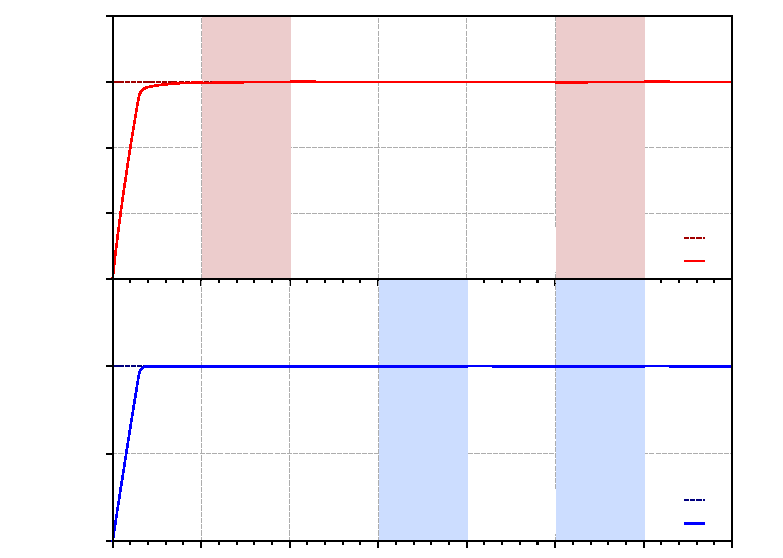
\includegraphics{fado}}%
    \gplfronttext
  \end{picture}%
\endgroup

\vspace{1cm}
\caption{Simulação da FADO com {\it offset} de -0,5 Volts.}
\label{fig:fado}
\end{figure}

\begin{figure}[htb]
\footnotesize
\centering
% GNUPLOT: LaTeX picture with Postscript
\begingroup
  \makeatletter
  \providecommand\color[2][]{%
    \GenericError{(gnuplot) \space\space\space\@spaces}{%
      Package color not loaded in conjunction with
      terminal option `colourtext'%
    }{See the gnuplot documentation for explanation.%
    }{Either use 'blacktext' in gnuplot or load the package
      color.sty in LaTeX.}%
    \renewcommand\color[2][]{}%
  }%
  \providecommand\includegraphics[2][]{%
    \GenericError{(gnuplot) \space\space\space\@spaces}{%
      Package graphicx or graphics not loaded%
    }{See the gnuplot documentation for explanation.%
    }{The gnuplot epslatex terminal needs graphicx.sty or graphics.sty.}%
    \renewcommand\includegraphics[2][]{}%
  }%
  \providecommand\rotatebox[2]{#2}%
  \@ifundefined{ifGPcolor}{%
    \newif\ifGPcolor
    \GPcolortrue
  }{}%
  \@ifundefined{ifGPblacktext}{%
    \newif\ifGPblacktext
    \GPblacktexttrue
  }{}%
  % define a \g@addto@macro without @ in the name:
  \let\gplgaddtomacro\g@addto@macro
  % define empty templates for all commands taking text:
  \gdef\gplbacktext{}%
  \gdef\gplfronttext{}%
  \makeatother
  \ifGPblacktext
    % no textcolor at all
    \def\colorrgb#1{}%
    \def\colorgray#1{}%
  \else
    % gray or color?
    \ifGPcolor
      \def\colorrgb#1{\color[rgb]{#1}}%
      \def\colorgray#1{\color[gray]{#1}}%
      \expandafter\def\csname LTw\endcsname{\color{white}}%
      \expandafter\def\csname LTb\endcsname{\color{black}}%
      \expandafter\def\csname LTa\endcsname{\color{black}}%
      \expandafter\def\csname LT0\endcsname{\color[rgb]{1,0,0}}%
      \expandafter\def\csname LT1\endcsname{\color[rgb]{0,1,0}}%
      \expandafter\def\csname LT2\endcsname{\color[rgb]{0,0,1}}%
      \expandafter\def\csname LT3\endcsname{\color[rgb]{1,0,1}}%
      \expandafter\def\csname LT4\endcsname{\color[rgb]{0,1,1}}%
      \expandafter\def\csname LT5\endcsname{\color[rgb]{1,1,0}}%
      \expandafter\def\csname LT6\endcsname{\color[rgb]{0,0,0}}%
      \expandafter\def\csname LT7\endcsname{\color[rgb]{1,0.3,0}}%
      \expandafter\def\csname LT8\endcsname{\color[rgb]{0.5,0.5,0.5}}%
    \else
      % gray
      \def\colorrgb#1{\color{black}}%
      \def\colorgray#1{\color[gray]{#1}}%
      \expandafter\def\csname LTw\endcsname{\color{white}}%
      \expandafter\def\csname LTb\endcsname{\color{black}}%
      \expandafter\def\csname LTa\endcsname{\color{black}}%
      \expandafter\def\csname LT0\endcsname{\color{black}}%
      \expandafter\def\csname LT1\endcsname{\color{black}}%
      \expandafter\def\csname LT2\endcsname{\color{black}}%
      \expandafter\def\csname LT3\endcsname{\color{black}}%
      \expandafter\def\csname LT4\endcsname{\color{black}}%
      \expandafter\def\csname LT5\endcsname{\color{black}}%
      \expandafter\def\csname LT6\endcsname{\color{black}}%
      \expandafter\def\csname LT7\endcsname{\color{black}}%
      \expandafter\def\csname LT8\endcsname{\color{black}}%
    \fi
  \fi
  \setlength{\unitlength}{0.0500bp}%
  \begin{picture}(7200.00,5040.00)%
    \gplgaddtomacro\gplbacktext{%
      \csname LTb\endcsname%
      \put(726,3150){\makebox(0,0)[r]{\strut{} 5}}%
      \csname LTb\endcsname%
      \put(726,3780){\makebox(0,0)[r]{\strut{} 10}}%
      \csname LTb\endcsname%
      \put(726,4409){\makebox(0,0)[r]{\strut{} 15}}%
      \csname LTb\endcsname%
      \put(726,5039){\makebox(0,0)[r]{\strut{} 20}}%
      \csname LTb\endcsname%
      \put(921,2237){\makebox(0,0){\strut{}}}%
      \csname LTb\endcsname%
      \put(1771,2237){\makebox(0,0){\strut{}}}%
      \csname LTb\endcsname%
      \put(2620,2237){\makebox(0,0){\strut{}}}%
      \csname LTb\endcsname%
      \put(3470,2237){\makebox(0,0){\strut{}}}%
      \csname LTb\endcsname%
      \put(4320,2237){\makebox(0,0){\strut{}}}%
      \csname LTb\endcsname%
      \put(5170,2237){\makebox(0,0){\strut{}}}%
      \csname LTb\endcsname%
      \put(6019,2237){\makebox(0,0){\strut{}}}%
      \csname LTb\endcsname%
      \put(6869,2237){\makebox(0,0){\strut{}}}%
      \put(352,3779){\rotatebox{-270}{\makebox(0,0){\strut{}Nível [cm]}}}%
    }%
    \gplgaddtomacro\gplfronttext{%
      \csname LTb\endcsname%
      \put(6278,2913){\makebox(0,0)[r]{\strut{}Ref. $T_1$}}%
      \csname LTb\endcsname%
      \put(6278,2693){\makebox(0,0)[r]{\strut{}Saída $T_1$}}%
    }%
    \gplgaddtomacro\gplbacktext{%
      \csname LTb\endcsname%
      \put(726,0){\makebox(0,0)[r]{\strut{} 0}}%
      \csname LTb\endcsname%
      \put(726,840){\makebox(0,0)[r]{\strut{} 10}}%
      \csname LTb\endcsname%
      \put(726,1680){\makebox(0,0)[r]{\strut{} 20}}%
      \csname LTb\endcsname%
      \put(726,2520){\makebox(0,0)[r]{\strut{} 30}}%
      \csname LTb\endcsname%
      \put(921,-283){\makebox(0,0){\strut{}0}}%
      \csname LTb\endcsname%
      \put(1771,-283){\makebox(0,0){\strut{}15}}%
      \csname LTb\endcsname%
      \put(2620,-283){\makebox(0,0){\strut{}30}}%
      \csname LTb\endcsname%
      \put(3470,-283){\makebox(0,0){\strut{}45}}%
      \csname LTb\endcsname%
      \put(4320,-283){\makebox(0,0){\strut{}60}}%
      \csname LTb\endcsname%
      \put(5170,-283){\makebox(0,0){\strut{}75}}%
      \csname LTb\endcsname%
      \put(6019,-283){\makebox(0,0){\strut{}90}}%
      \csname LTb\endcsname%
      \put(6869,-283){\makebox(0,0){\strut{}105}}%
      \put(352,1260){\rotatebox{-270}{\makebox(0,0){\strut{}Nível [cm]}}}%
      \put(3895,-613){\makebox(0,0){\strut{}Tempo [s]}}%
    }%
    \gplgaddtomacro\gplfronttext{%
      \csname LTb\endcsname%
      \put(6278,393){\makebox(0,0)[r]{\strut{}Ref. $T_2$}}%
      \csname LTb\endcsname%
      \put(6278,173){\makebox(0,0)[r]{\strut{}Saída $T_2$}}%
    }%
    \gplbacktext
    \put(0,0){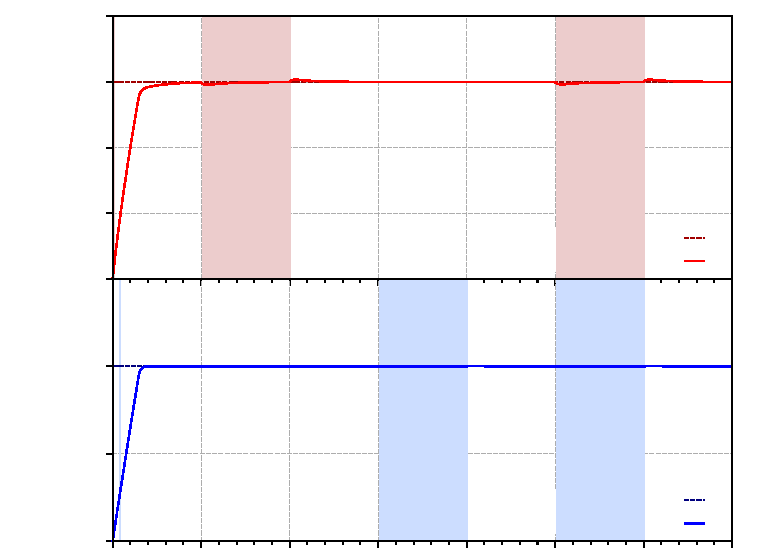
\includegraphics{favk}}%
    \gplfronttext
  \end{picture}%
\endgroup

\vspace{1cm}
\caption{Simulação da FAVK com $K_m$ reduzido a 75\% do valor original.}
\label{fig:favk}
\end{figure}

\begin{figure}[htb]
\footnotesize
\centering
% GNUPLOT: LaTeX picture with Postscript
\begingroup
  \makeatletter
  \providecommand\color[2][]{%
    \GenericError{(gnuplot) \space\space\space\@spaces}{%
      Package color not loaded in conjunction with
      terminal option `colourtext'%
    }{See the gnuplot documentation for explanation.%
    }{Either use 'blacktext' in gnuplot or load the package
      color.sty in LaTeX.}%
    \renewcommand\color[2][]{}%
  }%
  \providecommand\includegraphics[2][]{%
    \GenericError{(gnuplot) \space\space\space\@spaces}{%
      Package graphicx or graphics not loaded%
    }{See the gnuplot documentation for explanation.%
    }{The gnuplot epslatex terminal needs graphicx.sty or graphics.sty.}%
    \renewcommand\includegraphics[2][]{}%
  }%
  \providecommand\rotatebox[2]{#2}%
  \@ifundefined{ifGPcolor}{%
    \newif\ifGPcolor
    \GPcolortrue
  }{}%
  \@ifundefined{ifGPblacktext}{%
    \newif\ifGPblacktext
    \GPblacktexttrue
  }{}%
  % define a \g@addto@macro without @ in the name:
  \let\gplgaddtomacro\g@addto@macro
  % define empty templates for all commands taking text:
  \gdef\gplbacktext{}%
  \gdef\gplfronttext{}%
  \makeatother
  \ifGPblacktext
    % no textcolor at all
    \def\colorrgb#1{}%
    \def\colorgray#1{}%
  \else
    % gray or color?
    \ifGPcolor
      \def\colorrgb#1{\color[rgb]{#1}}%
      \def\colorgray#1{\color[gray]{#1}}%
      \expandafter\def\csname LTw\endcsname{\color{white}}%
      \expandafter\def\csname LTb\endcsname{\color{black}}%
      \expandafter\def\csname LTa\endcsname{\color{black}}%
      \expandafter\def\csname LT0\endcsname{\color[rgb]{1,0,0}}%
      \expandafter\def\csname LT1\endcsname{\color[rgb]{0,1,0}}%
      \expandafter\def\csname LT2\endcsname{\color[rgb]{0,0,1}}%
      \expandafter\def\csname LT3\endcsname{\color[rgb]{1,0,1}}%
      \expandafter\def\csname LT4\endcsname{\color[rgb]{0,1,1}}%
      \expandafter\def\csname LT5\endcsname{\color[rgb]{1,1,0}}%
      \expandafter\def\csname LT6\endcsname{\color[rgb]{0,0,0}}%
      \expandafter\def\csname LT7\endcsname{\color[rgb]{1,0.3,0}}%
      \expandafter\def\csname LT8\endcsname{\color[rgb]{0.5,0.5,0.5}}%
    \else
      % gray
      \def\colorrgb#1{\color{black}}%
      \def\colorgray#1{\color[gray]{#1}}%
      \expandafter\def\csname LTw\endcsname{\color{white}}%
      \expandafter\def\csname LTb\endcsname{\color{black}}%
      \expandafter\def\csname LTa\endcsname{\color{black}}%
      \expandafter\def\csname LT0\endcsname{\color{black}}%
      \expandafter\def\csname LT1\endcsname{\color{black}}%
      \expandafter\def\csname LT2\endcsname{\color{black}}%
      \expandafter\def\csname LT3\endcsname{\color{black}}%
      \expandafter\def\csname LT4\endcsname{\color{black}}%
      \expandafter\def\csname LT5\endcsname{\color{black}}%
      \expandafter\def\csname LT6\endcsname{\color{black}}%
      \expandafter\def\csname LT7\endcsname{\color{black}}%
      \expandafter\def\csname LT8\endcsname{\color{black}}%
    \fi
  \fi
  \setlength{\unitlength}{0.0500bp}%
  \begin{picture}(7200.00,5040.00)%
    \gplgaddtomacro\gplbacktext{%
      \csname LTb\endcsname%
      \put(726,3150){\makebox(0,0)[r]{\strut{} 5}}%
      \csname LTb\endcsname%
      \put(726,3780){\makebox(0,0)[r]{\strut{} 10}}%
      \csname LTb\endcsname%
      \put(726,4409){\makebox(0,0)[r]{\strut{} 15}}%
      \csname LTb\endcsname%
      \put(726,5039){\makebox(0,0)[r]{\strut{} 20}}%
      \csname LTb\endcsname%
      \put(921,2237){\makebox(0,0){\strut{}}}%
      \csname LTb\endcsname%
      \put(1771,2237){\makebox(0,0){\strut{}}}%
      \csname LTb\endcsname%
      \put(2620,2237){\makebox(0,0){\strut{}}}%
      \csname LTb\endcsname%
      \put(3470,2237){\makebox(0,0){\strut{}}}%
      \csname LTb\endcsname%
      \put(4320,2237){\makebox(0,0){\strut{}}}%
      \csname LTb\endcsname%
      \put(5170,2237){\makebox(0,0){\strut{}}}%
      \csname LTb\endcsname%
      \put(6019,2237){\makebox(0,0){\strut{}}}%
      \csname LTb\endcsname%
      \put(6869,2237){\makebox(0,0){\strut{}}}%
      \put(352,3779){\rotatebox{-270}{\makebox(0,0){\strut{}Level [cm]}}}%
    }%
    \gplgaddtomacro\gplfronttext{%
      \csname LTb\endcsname%
      \put(6278,2913){\makebox(0,0)[r]{\strut{}Setpoint $T_1$}}%
      \csname LTb\endcsname%
      \put(6278,2693){\makebox(0,0)[r]{\strut{}Output $T_1$}}%
    }%
    \gplgaddtomacro\gplbacktext{%
      \csname LTb\endcsname%
      \put(726,0){\makebox(0,0)[r]{\strut{} 0}}%
      \csname LTb\endcsname%
      \put(726,840){\makebox(0,0)[r]{\strut{} 10}}%
      \csname LTb\endcsname%
      \put(726,1680){\makebox(0,0)[r]{\strut{} 20}}%
      \csname LTb\endcsname%
      \put(726,2520){\makebox(0,0)[r]{\strut{} 30}}%
      \csname LTb\endcsname%
      \put(921,-283){\makebox(0,0){\strut{}0}}%
      \csname LTb\endcsname%
      \put(1771,-283){\makebox(0,0){\strut{}15}}%
      \csname LTb\endcsname%
      \put(2620,-283){\makebox(0,0){\strut{}30}}%
      \csname LTb\endcsname%
      \put(3470,-283){\makebox(0,0){\strut{}45}}%
      \csname LTb\endcsname%
      \put(4320,-283){\makebox(0,0){\strut{}60}}%
      \csname LTb\endcsname%
      \put(5170,-283){\makebox(0,0){\strut{}75}}%
      \csname LTb\endcsname%
      \put(6019,-283){\makebox(0,0){\strut{}90}}%
      \csname LTb\endcsname%
      \put(6869,-283){\makebox(0,0){\strut{}105}}%
      \put(352,1260){\rotatebox{-270}{\makebox(0,0){\strut{}Level [cm]}}}%
      \put(3895,-613){\makebox(0,0){\strut{}Time [s]}}%
    }%
    \gplgaddtomacro\gplfronttext{%
      \csname LTb\endcsname%
      \put(6278,393){\makebox(0,0)[r]{\strut{}Setpoint $T_2$}}%
      \csname LTb\endcsname%
      \put(6278,173){\makebox(0,0)[r]{\strut{}Output $T_2$}}%
    }%
    \gplbacktext
    \put(0,0){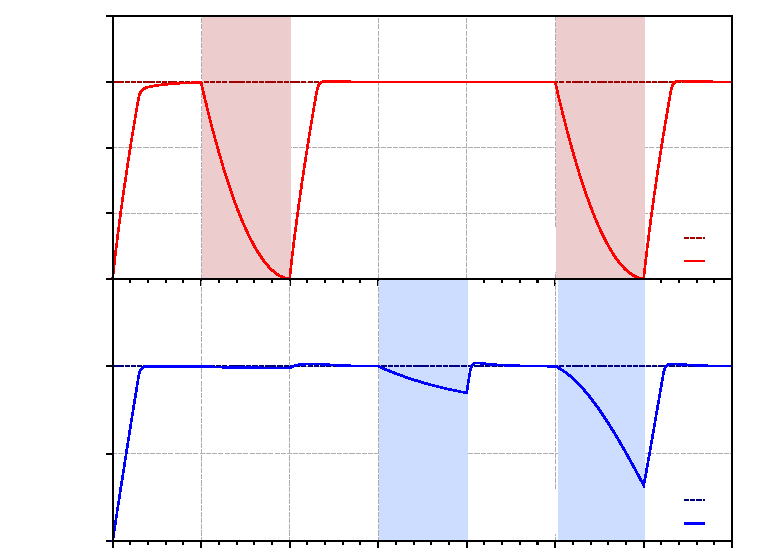
\includegraphics{faq}}%
    \gplfronttext
  \end{picture}%
\endgroup

\vspace{1cm}
\caption{Simulação da FAQ (Ganho = 0).}
\label{fig:faq}
\end{figure}

\begin{figure}[htb]
\footnotesize
\centering
% GNUPLOT: LaTeX picture with Postscript
\begingroup
  \makeatletter
  \providecommand\color[2][]{%
    \GenericError{(gnuplot) \space\space\space\@spaces}{%
      Package color not loaded in conjunction with
      terminal option `colourtext'%
    }{See the gnuplot documentation for explanation.%
    }{Either use 'blacktext' in gnuplot or load the package
      color.sty in LaTeX.}%
    \renewcommand\color[2][]{}%
  }%
  \providecommand\includegraphics[2][]{%
    \GenericError{(gnuplot) \space\space\space\@spaces}{%
      Package graphicx or graphics not loaded%
    }{See the gnuplot documentation for explanation.%
    }{The gnuplot epslatex terminal needs graphicx.sty or graphics.sty.}%
    \renewcommand\includegraphics[2][]{}%
  }%
  \providecommand\rotatebox[2]{#2}%
  \@ifundefined{ifGPcolor}{%
    \newif\ifGPcolor
    \GPcolortrue
  }{}%
  \@ifundefined{ifGPblacktext}{%
    \newif\ifGPblacktext
    \GPblacktexttrue
  }{}%
  % define a \g@addto@macro without @ in the name:
  \let\gplgaddtomacro\g@addto@macro
  % define empty templates for all commands taking text:
  \gdef\gplbacktext{}%
  \gdef\gplfronttext{}%
  \makeatother
  \ifGPblacktext
    % no textcolor at all
    \def\colorrgb#1{}%
    \def\colorgray#1{}%
  \else
    % gray or color?
    \ifGPcolor
      \def\colorrgb#1{\color[rgb]{#1}}%
      \def\colorgray#1{\color[gray]{#1}}%
      \expandafter\def\csname LTw\endcsname{\color{white}}%
      \expandafter\def\csname LTb\endcsname{\color{black}}%
      \expandafter\def\csname LTa\endcsname{\color{black}}%
      \expandafter\def\csname LT0\endcsname{\color[rgb]{1,0,0}}%
      \expandafter\def\csname LT1\endcsname{\color[rgb]{0,1,0}}%
      \expandafter\def\csname LT2\endcsname{\color[rgb]{0,0,1}}%
      \expandafter\def\csname LT3\endcsname{\color[rgb]{1,0,1}}%
      \expandafter\def\csname LT4\endcsname{\color[rgb]{0,1,1}}%
      \expandafter\def\csname LT5\endcsname{\color[rgb]{1,1,0}}%
      \expandafter\def\csname LT6\endcsname{\color[rgb]{0,0,0}}%
      \expandafter\def\csname LT7\endcsname{\color[rgb]{1,0.3,0}}%
      \expandafter\def\csname LT8\endcsname{\color[rgb]{0.5,0.5,0.5}}%
    \else
      % gray
      \def\colorrgb#1{\color{black}}%
      \def\colorgray#1{\color[gray]{#1}}%
      \expandafter\def\csname LTw\endcsname{\color{white}}%
      \expandafter\def\csname LTb\endcsname{\color{black}}%
      \expandafter\def\csname LTa\endcsname{\color{black}}%
      \expandafter\def\csname LT0\endcsname{\color{black}}%
      \expandafter\def\csname LT1\endcsname{\color{black}}%
      \expandafter\def\csname LT2\endcsname{\color{black}}%
      \expandafter\def\csname LT3\endcsname{\color{black}}%
      \expandafter\def\csname LT4\endcsname{\color{black}}%
      \expandafter\def\csname LT5\endcsname{\color{black}}%
      \expandafter\def\csname LT6\endcsname{\color{black}}%
      \expandafter\def\csname LT7\endcsname{\color{black}}%
      \expandafter\def\csname LT8\endcsname{\color{black}}%
    \fi
  \fi
  \setlength{\unitlength}{0.0500bp}%
  \begin{picture}(7200.00,5040.00)%
    \gplgaddtomacro\gplbacktext{%
      \csname LTb\endcsname%
      \put(726,3150){\makebox(0,0)[r]{\strut{} 5}}%
      \csname LTb\endcsname%
      \put(726,3780){\makebox(0,0)[r]{\strut{} 10}}%
      \csname LTb\endcsname%
      \put(726,4409){\makebox(0,0)[r]{\strut{} 15}}%
      \csname LTb\endcsname%
      \put(726,5039){\makebox(0,0)[r]{\strut{} 20}}%
      \csname LTb\endcsname%
      \put(921,2237){\makebox(0,0){\strut{}}}%
      \csname LTb\endcsname%
      \put(1771,2237){\makebox(0,0){\strut{}}}%
      \csname LTb\endcsname%
      \put(2620,2237){\makebox(0,0){\strut{}}}%
      \csname LTb\endcsname%
      \put(3470,2237){\makebox(0,0){\strut{}}}%
      \csname LTb\endcsname%
      \put(4320,2237){\makebox(0,0){\strut{}}}%
      \csname LTb\endcsname%
      \put(5170,2237){\makebox(0,0){\strut{}}}%
      \csname LTb\endcsname%
      \put(6019,2237){\makebox(0,0){\strut{}}}%
      \csname LTb\endcsname%
      \put(6869,2237){\makebox(0,0){\strut{}}}%
      \put(352,3779){\rotatebox{-270}{\makebox(0,0){\strut{}Nível [cm]}}}%
    }%
    \gplgaddtomacro\gplfronttext{%
      \csname LTb\endcsname%
      \put(6278,2913){\makebox(0,0)[r]{\strut{}Ref. $T_1$}}%
      \csname LTb\endcsname%
      \put(6278,2693){\makebox(0,0)[r]{\strut{}Saída $T_1$}}%
    }%
    \gplgaddtomacro\gplbacktext{%
      \csname LTb\endcsname%
      \put(726,0){\makebox(0,0)[r]{\strut{} 0}}%
      \csname LTb\endcsname%
      \put(726,840){\makebox(0,0)[r]{\strut{} 10}}%
      \csname LTb\endcsname%
      \put(726,1680){\makebox(0,0)[r]{\strut{} 20}}%
      \csname LTb\endcsname%
      \put(726,2520){\makebox(0,0)[r]{\strut{} 30}}%
      \csname LTb\endcsname%
      \put(921,-283){\makebox(0,0){\strut{}0}}%
      \csname LTb\endcsname%
      \put(1771,-283){\makebox(0,0){\strut{}15}}%
      \csname LTb\endcsname%
      \put(2620,-283){\makebox(0,0){\strut{}30}}%
      \csname LTb\endcsname%
      \put(3470,-283){\makebox(0,0){\strut{}45}}%
      \csname LTb\endcsname%
      \put(4320,-283){\makebox(0,0){\strut{}60}}%
      \csname LTb\endcsname%
      \put(5170,-283){\makebox(0,0){\strut{}75}}%
      \csname LTb\endcsname%
      \put(6019,-283){\makebox(0,0){\strut{}90}}%
      \csname LTb\endcsname%
      \put(6869,-283){\makebox(0,0){\strut{}105}}%
      \put(352,1260){\rotatebox{-270}{\makebox(0,0){\strut{}Nível [cm]}}}%
      \put(3895,-613){\makebox(0,0){\strut{}Tempo [s]}}%
    }%
    \gplgaddtomacro\gplfronttext{%
      \csname LTb\endcsname%
      \put(6278,393){\makebox(0,0)[r]{\strut{}Ref. $T_2$}}%
      \csname LTb\endcsname%
      \put(6278,173){\makebox(0,0)[r]{\strut{}Saída $T_2$}}%
    }%
    \gplbacktext
    \put(0,0){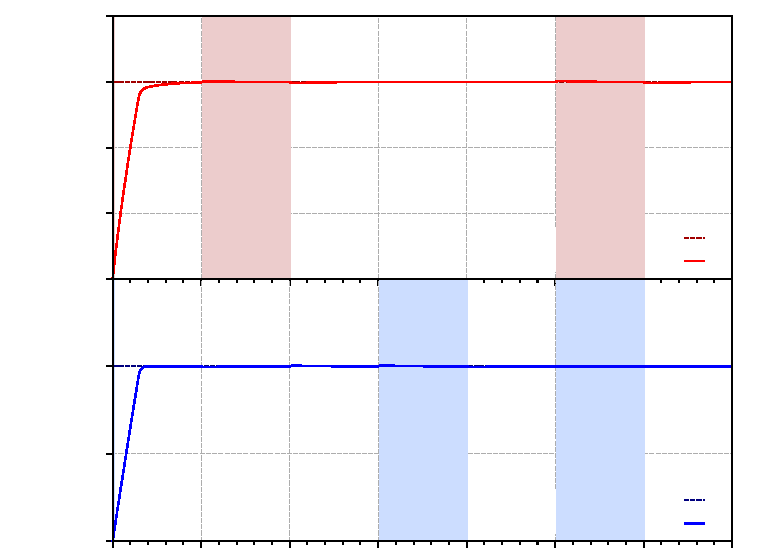
\includegraphics{fsivros}}%
    \gplfronttext
  \end{picture}%
\endgroup

\vspace{1cm}
\caption{Simulação da FSiVrOS com $a_i = a_{\tiny MED}/2$.}
\label{fig:fsivros}
\end{figure}

\begin{figure}[htb]
\footnotesize
\centering
% GNUPLOT: LaTeX picture with Postscript
\begingroup
  \makeatletter
  \providecommand\color[2][]{%
    \GenericError{(gnuplot) \space\space\space\@spaces}{%
      Package color not loaded in conjunction with
      terminal option `colourtext'%
    }{See the gnuplot documentation for explanation.%
    }{Either use 'blacktext' in gnuplot or load the package
      color.sty in LaTeX.}%
    \renewcommand\color[2][]{}%
  }%
  \providecommand\includegraphics[2][]{%
    \GenericError{(gnuplot) \space\space\space\@spaces}{%
      Package graphicx or graphics not loaded%
    }{See the gnuplot documentation for explanation.%
    }{The gnuplot epslatex terminal needs graphicx.sty or graphics.sty.}%
    \renewcommand\includegraphics[2][]{}%
  }%
  \providecommand\rotatebox[2]{#2}%
  \@ifundefined{ifGPcolor}{%
    \newif\ifGPcolor
    \GPcolortrue
  }{}%
  \@ifundefined{ifGPblacktext}{%
    \newif\ifGPblacktext
    \GPblacktexttrue
  }{}%
  % define a \g@addto@macro without @ in the name:
  \let\gplgaddtomacro\g@addto@macro
  % define empty templates for all commands taking text:
  \gdef\gplbacktext{}%
  \gdef\gplfronttext{}%
  \makeatother
  \ifGPblacktext
    % no textcolor at all
    \def\colorrgb#1{}%
    \def\colorgray#1{}%
  \else
    % gray or color?
    \ifGPcolor
      \def\colorrgb#1{\color[rgb]{#1}}%
      \def\colorgray#1{\color[gray]{#1}}%
      \expandafter\def\csname LTw\endcsname{\color{white}}%
      \expandafter\def\csname LTb\endcsname{\color{black}}%
      \expandafter\def\csname LTa\endcsname{\color{black}}%
      \expandafter\def\csname LT0\endcsname{\color[rgb]{1,0,0}}%
      \expandafter\def\csname LT1\endcsname{\color[rgb]{0,1,0}}%
      \expandafter\def\csname LT2\endcsname{\color[rgb]{0,0,1}}%
      \expandafter\def\csname LT3\endcsname{\color[rgb]{1,0,1}}%
      \expandafter\def\csname LT4\endcsname{\color[rgb]{0,1,1}}%
      \expandafter\def\csname LT5\endcsname{\color[rgb]{1,1,0}}%
      \expandafter\def\csname LT6\endcsname{\color[rgb]{0,0,0}}%
      \expandafter\def\csname LT7\endcsname{\color[rgb]{1,0.3,0}}%
      \expandafter\def\csname LT8\endcsname{\color[rgb]{0.5,0.5,0.5}}%
    \else
      % gray
      \def\colorrgb#1{\color{black}}%
      \def\colorgray#1{\color[gray]{#1}}%
      \expandafter\def\csname LTw\endcsname{\color{white}}%
      \expandafter\def\csname LTb\endcsname{\color{black}}%
      \expandafter\def\csname LTa\endcsname{\color{black}}%
      \expandafter\def\csname LT0\endcsname{\color{black}}%
      \expandafter\def\csname LT1\endcsname{\color{black}}%
      \expandafter\def\csname LT2\endcsname{\color{black}}%
      \expandafter\def\csname LT3\endcsname{\color{black}}%
      \expandafter\def\csname LT4\endcsname{\color{black}}%
      \expandafter\def\csname LT5\endcsname{\color{black}}%
      \expandafter\def\csname LT6\endcsname{\color{black}}%
      \expandafter\def\csname LT7\endcsname{\color{black}}%
      \expandafter\def\csname LT8\endcsname{\color{black}}%
    \fi
  \fi
  \setlength{\unitlength}{0.0500bp}%
  \begin{picture}(7200.00,5040.00)%
    \gplgaddtomacro\gplbacktext{%
      \csname LTb\endcsname%
      \put(726,3150){\makebox(0,0)[r]{\strut{} 5}}%
      \csname LTb\endcsname%
      \put(726,3780){\makebox(0,0)[r]{\strut{} 10}}%
      \csname LTb\endcsname%
      \put(726,4409){\makebox(0,0)[r]{\strut{} 15}}%
      \csname LTb\endcsname%
      \put(726,5039){\makebox(0,0)[r]{\strut{} 20}}%
      \csname LTb\endcsname%
      \put(921,2237){\makebox(0,0){\strut{}}}%
      \csname LTb\endcsname%
      \put(1771,2237){\makebox(0,0){\strut{}}}%
      \csname LTb\endcsname%
      \put(2620,2237){\makebox(0,0){\strut{}}}%
      \csname LTb\endcsname%
      \put(3470,2237){\makebox(0,0){\strut{}}}%
      \csname LTb\endcsname%
      \put(4320,2237){\makebox(0,0){\strut{}}}%
      \csname LTb\endcsname%
      \put(5170,2237){\makebox(0,0){\strut{}}}%
      \csname LTb\endcsname%
      \put(6019,2237){\makebox(0,0){\strut{}}}%
      \csname LTb\endcsname%
      \put(6869,2237){\makebox(0,0){\strut{}}}%
      \put(352,3779){\rotatebox{-270}{\makebox(0,0){\strut{}Level [cm]}}}%
    }%
    \gplgaddtomacro\gplfronttext{%
      \csname LTb\endcsname%
      \put(6278,2913){\makebox(0,0)[r]{\strut{}Setpoint $T_1$}}%
      \csname LTb\endcsname%
      \put(6278,2693){\makebox(0,0)[r]{\strut{}Output $T_1$}}%
    }%
    \gplgaddtomacro\gplbacktext{%
      \csname LTb\endcsname%
      \put(726,0){\makebox(0,0)[r]{\strut{} 0}}%
      \csname LTb\endcsname%
      \put(726,840){\makebox(0,0)[r]{\strut{} 10}}%
      \csname LTb\endcsname%
      \put(726,1680){\makebox(0,0)[r]{\strut{} 20}}%
      \csname LTb\endcsname%
      \put(726,2520){\makebox(0,0)[r]{\strut{} 30}}%
      \csname LTb\endcsname%
      \put(921,-283){\makebox(0,0){\strut{}0}}%
      \csname LTb\endcsname%
      \put(1771,-283){\makebox(0,0){\strut{}15}}%
      \csname LTb\endcsname%
      \put(2620,-283){\makebox(0,0){\strut{}30}}%
      \csname LTb\endcsname%
      \put(3470,-283){\makebox(0,0){\strut{}45}}%
      \csname LTb\endcsname%
      \put(4320,-283){\makebox(0,0){\strut{}60}}%
      \csname LTb\endcsname%
      \put(5170,-283){\makebox(0,0){\strut{}75}}%
      \csname LTb\endcsname%
      \put(6019,-283){\makebox(0,0){\strut{}90}}%
      \csname LTb\endcsname%
      \put(6869,-283){\makebox(0,0){\strut{}105}}%
      \put(352,1260){\rotatebox{-270}{\makebox(0,0){\strut{}Level [cm]}}}%
      \put(3895,-613){\makebox(0,0){\strut{}Time [s]}}%
    }%
    \gplgaddtomacro\gplfronttext{%
      \csname LTb\endcsname%
      \put(6278,393){\makebox(0,0)[r]{\strut{}Setpoint $T_2$}}%
      \csname LTb\endcsname%
      \put(6278,173){\makebox(0,0)[r]{\strut{}Output $T_2$}}%
    }%
    \gplbacktext
    \put(0,0){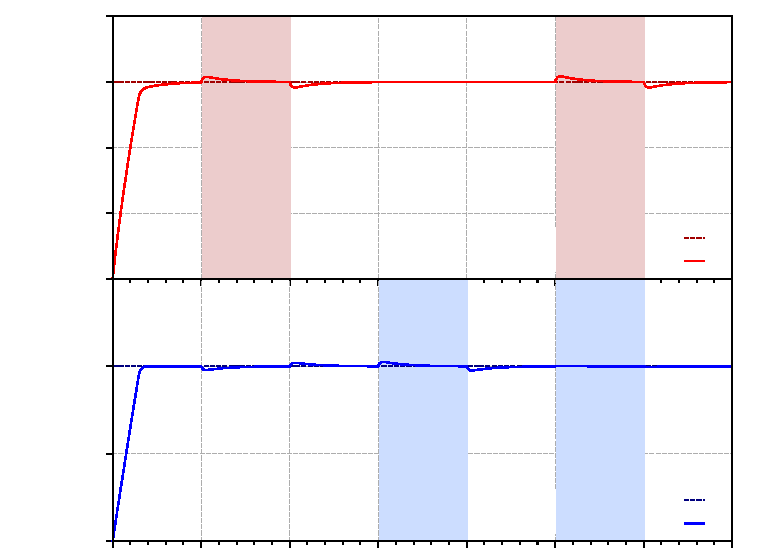
\includegraphics{fsieos}}%
    \gplfronttext
  \end{picture}%
\endgroup

\vspace{1cm}
\caption{Simulação da FSiEOS com $a_i = a_{\tiny MED}/4$.}
\label{fig:fsieos}
\end{figure}

Uma última observação pode ser feita a respeito da FSeQ, em que há a detecção da
falha em $T_1$ em um pequeno intervalo no final da simulação. Essa detecção
entretanto não comprometeu o funcionamento do sistema nos intervalos em que a
falha deveria realmente ser detectada. Trata-se, portanto, de um falso positivo.

Como dito anteriormente, as situações adversas podem ter ocorrido no sistema em
virtude do treinamento ter sido realizado co valores constantes para os
parâmetros. Por esse motivo os resultados obtidos nem sempre estão de acordo com
os valores da Tab. \ref{tab:melhores_redes_detec}.

% TODO CONCLUSAO?
%Apesar do número de acertos obtidos em algumas falhas durante o processo de
%validação, utilizando um sinal de excitação pseudo aleatório, percebeu-se que em
%casos mais simples, tais como a modificação do parâmetro para um valor
%constante, nem sempre o percentual de acerto era mantido. Um exemplo desse fato
%ocorre com a FSeDG, em que o percentual de erro salta de 2,12\% para X\%.

% ------------------------------------------------------------------------------
% TODO Dissertação
% \section{Comparação das propostas de detecção}

